\chapter{$B_s\to D_sl\nu$ Form Factors at All Physical $q^2$ from Heavy-HISQ}
\label{chap:BsDs}

In this chapter, I present the second of our two heavy-HISQ studies, the calculation of the $B_s\to D_sl\nu$ form factors $f^s_0(q^2)$ and $f^s_+(q^2)$ throughout all physical $q^2$, as defined in Sec. \ref{sec:weakdecays}. Like for $h_{A_1}^s(1)$, I'm giving this quantity the superscript $s$ to differentiate it from the more often referred to form factors for $B\to Dl\nu$ decays.

I briefly review the definition of the form factors here for ease of reading. The differential decay rate for $B_s\to D_s l \nu$ decays are given in the SM by \cite{PhysRevD.98.030001}:
\begin{align}
  &{d\Gamma\over dq^2} = \eta_{\text{EW}} { G_F^2 |V_{cb}|^2\over 24 \pi^3 M_{B_s}^2 } \left( 1 - {m_l^2\over q^2}\right)^2 |{\bf{p}}_{D_s}| \,\,\times \\
  \label{eq:branchingfraction}
  &\left[ \left( 1 + {m_l^2\over 2q^2}\right) M_{B_s}^2 |{\bf{p}}_{D_s}|^2 f_+^{s\,2}(q^2) + {3m_l^2\over 8q^2} (M_{B_s}^2-M_{D_s}^2)^2 f_0^{s\,2}(q^2) \right] \nonumber
\end{align}
where $m_l$ is the mass of the lepton, $\eta_{\text{EW}}$ is the electroweak correction \cite{SIRLIN198283,Ginsberg1968,PhysRevD.41.1736}, $q^2 = (p_{B_s} - p_{D_s})^2$ is the momentum transfer, and $f_0^s(q^2)$, $f_+^s(q^2)$ are the scalar and vector form factors that parameterize the non-perturbative contribution to the decay. The allowed range of $q^2$ values if the final states are on-shell is
\begin{align}
  m_l^2 \leq q^2 \leq (M_{B_s}-M_{D_s})^2.
\end{align}
The form factors parameterize matrix elements of the electroweak current between $B_s$ and $D_s$ states, $\langle D_s | (V-A)_{\mu} | B_s \rangle$ where $V_{\mu}=\bar{b}\gamma_{\mu}c$ is the vector component and $A_{\mu}=\bar{b}\gamma_5\gamma_{\mu} c$ is the axial vector component. In a pseudoscalar-to-pseudoscalar amplitude, only $V_{\mu}$ contributes, since $\langle D_s | A_{\mu} | B_s \rangle$ does not satisfy the parity invariance of QCD. The vector current in terms of form factors is given by
\begin{align}
  \langle D_s | V^{\mu} | B_s \rangle &= f_+^s(q^2) \left[ p_{B_s}^{\mu} + p_{D_s}^{\mu} - {M_{B_s}^2 - M_{D_s}^2 \over q^2} q^{\mu} \right] \nonumber \\
  &+ f_0^s(q^2) { M_{B_s}^2 - M_{D_s}^2 \over q^2} q^{\mu}\,.
  \label{eq:vectorcurrent}
\end{align}
Analyticity of this matrix element demands that
\begin{align}
  f_+^s(0) = f_0^s(0)\,.
  \label{eq:q20constraint}
\end{align}
Via the PCVC relation, the form factor $f_0^s(q^2)$ is also directly related to the matrix element of the scalar current $S=\bar{b}c\,$:
\begin{align}
  (m_b-m_c)\langle D_s | S | B_s \rangle = (M^2_{B_s} - M^2_{D_s}) f_0^s(q^2)\,.
    \label{eq:scalarcurrent}
\end{align}
In our calculation we access the form factors by computing matrix elements of the temporal vector current $V_0$ and the scalar current $S$. The form factors can be extracted from this combination using expresions derived from equations \eqref{eq:vectorcurrent} and \eqref{eq:scalarcurrent}:
\begin{align}
  f_0^s(q^2) &= {m_b - m_c\over M_{B_s}^2 - M_{D_s}^2 } \langle D_s | S | B_s \rangle, \\
  f_+^s(q^2) &= {1\over 2M_{B_s}} { \delta^M \langle D_s | S | B_s \rangle - q^2 \langle D_s | V_0 | B_s \rangle \over {\bf{p}}^2_{D_s}}, \\
    &( \, \delta^M = (m_b - m_c)(M_{B_s}-E_{D_s}) \, ). \nonumber
\end{align}

Our goal is to compute $f_0^s(q^2)$ and $f_+^s(q^2)$ throughout the range of $q^2$ values $0 \leq q^2 \leq (M_{B_s}-M_{D_s})^2 \equiv q^2_{\text{max}}$. We extend the range to $q^2=0$ in order to take advantage of the constraint in Eq. \eqref{eq:q20constraint}. To achieve this, we compute $\langle D_s | S | H_s \rangle$ and $\langle D_s | V_0 | H_s \rangle$ on the lattice, where the $H_s$ meson is at rest and $D_s$ mesons are given an appropriate array of spatial momenta.

%Those interested in simply using the form factors calculated here should refer to Sec. \ref{sec:reconstructing_formfactors}, which gives all information necessary for reconstructing our form factors.

\section{Motivation}
\label{sec:BsDs_intro}

%% The decays of heavy measons like the $B$ and $B_s$ is a potential source of insights into physics beyond the Standard Model (SM). Namely, quark flavour-changing $B$ decays have gained much interest due to a number of related tensions between experimental measurements and SM predictions \cite{Wei:2009zv,Lees:2012xj,Lees:2012tva,Lees:2013uzd,Aaij:2014pli,Aaij:2014ora,Huschle:2015rga,Aaij:2015oid,Aaij:2015yra,Aaij:2015xza,Aaij:2016flj,Wehle:2016yoi,Sato:2016svk,Hirose:2017dxl,Aaij:2017deq,Aaij:2017uff,Aaij:2017vbb,Sirunyan:2017dhj,Aaboud:2018krd}.
%Discrepancies between systematically independent determinations of Cabibbo-Kobayashi-Maskawa (CKM) matrix elements \cite{Amhis:2016xyh,Bevan:2014iga,Alberti:2014yda} have also sparked interest. 

$B_s\to D_s l\nu$ decays can supply a new method for precisely determining the CKM element $|V_{cb}|$. Determination of $|V_{cb}|$ in this way requires both a measurement of the branching fraction and a theoretical determination of the form factors, as explained in Sec. \ref{sec:weakdecays}. To obtain the highest possible precision, data for both the form factors and branching fractions are required throughout the largest possible range of momentum transfer. Analogous approaches were already performed using $B\to D l \nu$ decays \cite{Buskulic:1996yq,Bartelt:1998dq,Aubert:2008yv,Aubert:2009ac,Lattice:2015rga,Na:2015kha,Glattauer:2015teq}. 

The $B_s\to D_s l\nu$ decay can also supply a new test of the SM, by comparing the theoretical and experimental determinations of the ratio $R_{D_s}$, defined in Eq. \eqref{eq:Rratios}. This would be especially illuminating since tension has been found in the intimately related ratios $R_{D^{(*)}}$. The presence or absence of an anomaly in $R_{D_s}$ would help to confirm or dismiss a new physics explanation for such a family of anomalies.

The $B_s\to D_s l\nu$ scalar form factor is useful in the experimental extraction of $B_s \to \mu^+\mu^-$ branching fractions. Taking a ratio of the $B_s\to D_s$ and $B\to D$ scalar form factors gives the so-called fragmentation ratio, the ratio of probabilities of a $b$ quark hadronizing into a $B$ or $B_s$ meson. In analyses such as \cite{CMS:2014xfa}, $B_s \to \mu^+\mu^-$ branching fractions are measured using $B_u^+\to J/\psi(\mu^+\mu^-)K^+$ and $B_d^0\to K^+\pi_-$ as normalization channels, in this case one requires a value for the fragmentation ratio.

Similar to the $B_{(s)}\to D_{(s)}^*$ case, chiral perturbation theory implies that form factors for $B_s \to D_s$ and $B \to D$ decays are insensitive to the mass of the spectator quark, implying that form factors for these two decays are approximately equal \cite{Laiho:2005ue}. This expectation has been validated by previous lattice calculations, for example in \cite{PhysRevD.85.114502} the ratio of scalar form factors for the two decays at momentum transfer $q^2=M^2_{\pi}$ was found to be $f^s_0(M_{\pi}^2)/f_0(M_{\pi}^2) = 1.054(50)$, while \cite{Monahan:2017uby} found the value $f^s_0(M_{\pi}^2)/f_0(M_{\pi}^2) = 1.006(62)$. Hence we can expect to learn about $B\to D$ form factors by studying $B_s\to D_s$. 

While $B\to D$ form factors are currently more phenomenologically useful, $B_s\to D_s$ form factors are more attractive on the lattice QCD side. The absence of valence light ($u$ or $d$) quarks means lattice QCD results have smaller statistical errors, are less computationally expensive, have a more simple chiral extrapolation to the physical light mass, and negligible finite volume effects. This makes the $B_s \to D_s l\nu$ decay a useful test bed for lattice techniques that may be later used to study $B \to D l \nu$ decays.

A number of lattice calculations of $B_{(s)} \to D_{(s)}$ form factors have already been performed. The FNAL/MILC collaboration produced $B\to D$ form factors on the $N_f=2+1$ MILC gluon ensembles using the Fermilab action for $b$ and $c$ valence quarks and ASQTAD light quarks \cite{Lattice:2015rga}. They also, in an earler work, computed the ratio of scalar form factors for $B_s\to D_s$ and $B\to D$ to obtain the fragmentation ratio \cite{PhysRevD.85.114502}. The HPQCD collaboration computed both $B\to D$ and $B_s\to D_s$ form factors on the $N_f=2+1$ MILC gluon ensembles using the NRQCD action for the valence $b$, and the HISQ action for all other quarks \cite{Na:2015kha,Monahan:2017uby}. Atoui et. al. also produced $B_s\to D_s$ form factors using maximally twisted Wilson quarks on $N_f=2$ gluon ensembles \cite{Atoui2014}. A calculaton of the $B_s\to D_s$ form factors by the RBC/UKQCD collaboration is currently underway \cite{RBCmichigan}.

A considerable limitation in the FNAL/MILC and HPQCD studies is the requirement for perturbative matching between the lattice effective field theories and continuum QCD. FNAL/MILC required a matching that was only available to 1-loop, resulting in an $\mathcal{O}(\alpha_s^2)$ systematic error. In the HPQCD calculation, NRQCD-HISQ currents were truncated, prompting them to report large systematic errors. Besides the reported errors, as was discussed in Chapter \ref{chap:nrqcd}, parts of the NRQCD-HISQ vector current that contribute away from zero recoil have a large magnitude ($\sim 30\%$ of the leading order). The currents used in this study did not take these large subleading currents into account, so the result from this may have large uncontrolled systematic errors.

Another limitation present in each of the aforementioned studies is that the lattice data is limited to a region of high $q^2$. To generate lattice points at lower $q^2$, a large spatial momentum must be given to one of the quarks on the lattice. Due to signal/noise degradation, adding momentum leads to an exponential increase of noise in correlation functions. Hence, in cases like $B_{(s)}\to D_{(s)}$, lattice data close to $q^2=0$ would be uselessly noisy. Lattice results must be limited to high $q^2$. This fact necessitates an extrapolation from the data in the high $q^2$ region to the rest of the physical range. Since there has been some controversy in choices of form factor extrapolations through $q^2$ recently (for example see \cite{Bigi:2017njr,Grinstein:2017nlq}), it would be desirable to instead have lattice data covering the entire $q^2$ range. We can in fact achieve this with the heavy-HISQ approach. This is because in heavy-HISQ the $b$ quarks are lighter than physical, this shrinks the $q^2$ range, meaning smaller spatial momenta are required to cover the range.


\section{Calculation Details}
\label{sec:lattice}

\subsection{Lattice Setup}

%% \begin{table*}[htb!]
%%   \begin{center}
%%     \begin{tabular}{c c c c c c c c c c}
%%       \hline
%%       set & handle & $a/$fm  & $N_x^3\times N_t$ & $am_{l0}$ & $am_{s0}$ & $am_{c0}$  \\ [0.5ex]
%%       \hline
%%       1 & \bf{fine} & 0.0884(6) & $32^3\times96$ & 0.0074 & 0.037 & 0.440 \\ [1ex]
%%       2 & \bf{fine-physical} & 0.0873(5) & $64^3\times96$ & 0.0012 & 0.0363 & 0.432 \\ [1ex]
%%       3 & \bf{superfine} & 0.05922(12) & $48^3\times144$ & 0.0048 & 0.024 & 0.286 \\ [1ex]
%%       4 & \bf{ultrafine} & 0.04406(23) &  $64^3\times192$ & 0.00316 & 0.0158 & 0.188  \\ [1ex]
%%       \hline
%%     \end{tabular}
%%   \end{center}
%%     \caption{Parameters for gluon ensembles \cite{Bazavov:2010ru,Bazavov:2012xda}. $a$ is the lattice spacing, values for sets 1 \& 2 deduced in \cite{Dowdall:2013rya}, set 3 from \cite{Chakraborty:2014aca}. We thank C. McNeile for computing the $a$ value on set 4. These $a$ values are determined by measuring the Wilson flow parameter $w_0/a$ on the lattice, then using the known value for $w_0$ to isolate $a$. $N_x$ is the spatial extent and $N_t$ the temporal extent of the lattice. Light, strange and charm quarks are included in the sea, their masses are given in columns 5-7. \label{tab:ensembles}}
%% \end{table*}

%% \begin{table*}[htb!]
%%   \begin{center}
%%     \begin{tabular}{c c c c c c c c c c}
%%       \hline
%%       set & $am_{s0}^{\text{val}}$ & $am_{c0}^{\text{val}}$ & $am^{\text{val}}_{h0}$ & $|a{\bf{p}}_{D_s}|$ & $\theta$ & $T$ \\ [0.5ex]
%%       \hline
%%       1 & 0.0376 & 0.45
%%       & 0.5 & 0, 0.056 & 0, 0.328 & 14, 17, 20 \\ [1ex]
%%       & & & 0.65 & 0, 0.142, 0.201 & 0, 0.833, 1.181 & \\ [1ex]
%%       & & & 0.8 & 0, 0.227, 0.323 & 0, 1.334, 1.900 & \\ [1ex]

%%       \hline
%%       2 & 0.036 & 0.433
%%       & 0.5 & 0, 0.0279 & 0, 0.328 & 14, 17, 20 \\ [1ex]
%%       & & & 0.8 & 0, 0.162 & 0, 1.900 & \\ [1ex]

%%       \hline
%%       3 & 0.0234 & 
%%       0.274 & 0.427 & 0, 0.113, 0.161 &  0, 0.998, 1.417  & 22, 25, 28 \\ [1ex]
%%       & & & 0.525 & 0, 0.161, 0.244 & 0, 1.417, 2.151  & \\ [1ex]
%%       & & & 0.65 & 0, 0.244, 0.338 & 0, 2.151, 2.978  & \\ [1ex]
%%       & & & 0.8 & 0, 0.338, 0.438 & 0, 2.978, 3.862  & \\ [1ex]

%%       \hline
%%       4 & 0.0165 
%%       & 0.194 & 0.5 & 0, 0.202, 0.281 & 0, 2.38, 3.306 & 31, 36, 41 \\ [1ex]
%%       & & & 0.65 & 0, 0.202, 0.281, 0.382 & 0, 2.38, 3.306, 4.494  & \\ [1ex]
%%       & & & 0.8 & 0, 0.281, 0.382, 0.473 & 0, 3.306, 4.494, 5.562  & \\ [1ex]
%%       \hline
%%     \end{tabular}
%%   \end{center}
%%   \caption{}
%%   \label{tab:ensembles}
%% \end{table*}

\begin{table*}[htb!]
  \begin{center}
    \begin{tabular}{c c c c c c c c c c}
      \hline
      set & $am_{s0}^{\text{val}}$ & $am_{c0}^{\text{val}}$ & $am^{\text{val}}_{h0}$ & $|a{\bf{p}}_{D_s}|$ & $T/a$ \\ [0.5ex]
      \hline
      1 & 0.0376 & 0.45
      & 0.5 & 0, 0.056 & 14, 17, 20 \\ [1ex]
      & & & 0.65 & 0, 0.142, 0.201 &  \\ [1ex]
      & & & 0.8 & 0, 0.227, 0.323 &  \\ [1ex]

      \hline
      2 & 0.036 & 0.433
      & 0.5 & 0, 0.0279 & 14, 17, 20 \\ [1ex]
      & & & 0.8 & 0, 0.162  & \\ [1ex]

      \hline
      3 & 0.0234 & 
      0.274 & 0.427 & 0, 0.113, 0.161 & 22, 25, 28 \\ [1ex]
      & & & 0.525 & 0, 0.161, 0.244 & \\ [1ex]
      & & & 0.65 & 0, 0.244, 0.338 & \\ [1ex]
      & & & 0.8 & 0, 0.338, 0.438 & \\ [1ex]

      \hline
      4 & 0.0165 
      & 0.194 & 0.5 & 0, 0.202, 0.281 & 31, 36, 41 \\ [1ex]
      & & & 0.65 & 0, 0.202, 0.281, 0.382 & \\ [1ex]
      & & & 0.8 & 0, 0.281, 0.382, 0.473 & \\ [1ex]
      \hline
    \end{tabular}
  \end{center}
  \caption{Simulation details. Columns 2 and 3 give the $s$ and $c$ valence quark masses, which were tuned in \cite{Chakraborty:2014aca}. Column 4 gives the bare heavy quark masses, we use a number of heavy quark masses to assist the extrapolation to the physical $b$ mass. Column 5 gives the absolute value of the spatial momentum given to the $D_s$ meson, using a momentum twist, in lattice units. These values were chosen with the following rationale: when only 2 are used, these correspond to the $q^2=0$ and $q^2_{\text{max}}\,$ points (except on the fine-physical ensemble, where we compute at the points $q^2_{\text{max}}$ and $q^2_{\text{max}}/2$). When 3 twists are used, the momenta correspond to $q^2=0$, $q^2=q^2_{\text{max}}/2$, and $q^2_{\text{max}}$ points. When 4 are used, these are points for $q^2_{\text{max}}$, $3q^2_{\text{max}}/4$, $q^2_{\text{max}}/2$, $q^2_{\text{max}}/4$, $q^2=0$. To give the $D_s$ meson these spatial momenta we gave the charm an appropriate momentum twist in the $(1,1,1)$ direction. Column 6 gives the temporal separations between source and sink, $T$, of the 3-point correlation functions computed on each ensemble.}
  \label{tab:simulation}
\end{table*}

This calculation closely followed the approach employed in our calculation of the $B_s\to D_s^*$ axial form factor at zero recoil, given in the last chapter. The main modifications required for this calculation were 1) the form factors are not protected by Luke's theorem, so a more general fit form for the extrapolation in $m_h$ was required, and 2) to cover the $q^2$ range we gave the charm quark a number of spatial momentum values via a momentum twist (Sec. \ref{sec:momentum_twist}) and interpolated the results to all $q^2$.

We used the same set of ensembles as in the $B_s\to D_s^*$ study. In three of the four ensembles (sets 2, 4 and 5), the bare light mass is set to $m_{l0}/m_{s0} = 0.2$. The fact that the $m_{l0}$ value is unphysically high is expected to have a small effect on the form factors, due to the lack of valence light quarks, and previous experience of the form factor dependence on $m_{l0}$ \cite{Monahan:2017uby}. The small effect due to the unphysical $m_{l0}$ is quantified by including a fourth ensemble (set 3) with roughly physical $m_{l0}$, and corrected for. 

We used a number of different masses for the valence heavy quark $am_{h0}^{\text{val}}$. Unphysically light $h$-quarks reduce the $q^2$ range, meaning we can obtain lattice data at both ends of the range while the statistical noise remains under control, unlike previous studies of these form factors.

As detailed in Sec. \ref{sec:staggeredcorrelators}, staggered correlation functions are built by a combination of staggered propagators $g(x,y)$ and staggered phases. In this calculation we only need local (non-point-split) operators, this is an advantage since point-split operators lead to correlation functions noisier than those using local operators.

We computed a number of correlation functions on each ensemble. Valence masses, momenta and other inputs to the calculation are given in Table \ref{tab:simulation}. First, we computed 2-point correlation functions between eigenstates of momentum ${\textbf{p}}$, objects of the form
\begin{align}
  C_{M}({\textbf{p}},t) =& \langle \tilde{\Phi}_M ({\bf{p}},t) \tilde{\Phi}_M^{\dagger}({\bf{p}},0) \rangle, \\ 
  &\tilde{\Phi}_M({\bf{p}},t) = \sum_{{\bf{x}}} e^{-i\bf{p}\cdot \bf{x}} \bar{q}({\bf{x}},t) \Gamma q'({\bf{x}},t), \nonumber
\end{align}
where $\langle \rangle$ represents a functional integral over all fields, $q,q'$ are valence quark fields of the flavours the $M$ meson is charged under, and $\Gamma$ is the spin-taste structure of $M$. We computed these for all $t$ values, i.e. $0\leq t \leq N_t$.

%% In some cases, momentum was given to the meson by imposing twisted boundary conditions on the gluon fields when computing propagators, as described in Sec. \ref{sec:momentum_twist}.

%To generate these correlators we use random wall sources, and use extended sources for the 3-point correlation functions, as described in Sec. IV of \cite{Na:2010uf}.

We computed correlation functions for a heavy-strange pseudoscalar, $H_s$, with spin-taste structure $(\gamma_5\otimes \gamma_5)$, at rest. In terms of staggered propagators, this takes the form
\begin{align}
  C_{H_s}({\textbf{0}},t) = \sum_{\bf{x},\bf{y}} \left\langle \text{Tr}\left[ g_h(x,y) g_s^{\dagger}(x,y) \right] \right\rangle,
  \label{eq:pseudoscalar_corrs}
\end{align}
where $g_q(x,y)$ is a staggered propagator for flavour $q$, and the trace is over color. Here $x_0=0$ and $y_0=t$. We also computed correlators for a charm-strange pseudoscalar meson $D_s$, with structure $(\gamma_{\mu}\otimes \gamma_{\mu})$ and momentum ${\bf{p}}$, using
\begin{align}
  C_{D_s}({\textbf{p}},t) = \sum_{\bf{x},\bf{y}} \left\langle \text{Tr}\left[ g^{\theta_{\textbf{p}}}_c(x,y) g_s^{\dagger}(x,y) \right] \right\rangle,
\end{align}
where $g_q^{\theta_{\textbf{p}}}(x,y)$ denotes a propagator with momentum twist $\theta_{\textbf{p}}$ correpsonding to momentum ${\textbf{p}}$. We computed this using a number of twists to produce the range of momenta given in Table \ref{tab:simulation}. We designed the $c$ propagators to have momentum $a{\bf{p}} = |a{\bf{p}}|(1,1,1)$, by imposing a twist $\theta = N_x |a{\bf{p}}| / \pi \sqrt{3}$ in each spatial direction.

We also computed non-goldstone pseudoscalar heavy-strange mesons at rest, denoted $\hat{H}_s$. These are necessary for extracting the vector current. This has spin-taste structure $(\gamma_0\gamma_5\otimes \gamma_0\gamma_5)$. $\hat{H}_s$ correlators were computed using
\begin{align}
  C_{\hat{H}_s}(t) = \sum_{\bf{x},\bf{y}}(-1)^{\bar{x}_0+\bar{y}_0} \left\langle \text{Tr}\left[ g_h(x,y) g^{\dagger}_s(x,y) \right] \right\rangle,
\end{align}
where I use the notation $\bar{z}_{\mu} = \sum_{\nu\neq\mu} z_{\nu}$.

We also computed correlators for $H_c$ mesons, heavy-charmed pseudoscalars, using the same form as the $H_s$ correlator (Eq. \eqref{eq:pseudoscalar_corrs}). This is used to find $H_c$ decay constants, these are useful in our continuum and $m_h$ extrapolation.

The heavy-mass extrapolation requires masses of $\eta_h$ mesons, heavy-heavy pseudoscalars artificially forbidden to annihilate. To quantify mistuning of the charm and strange quark masses, we also required masses for $\eta_c$ and $\eta_s$ mesons, identical to $\eta_h$ with $h$ replaced $c$ and $s$ quarks respectively. We computed correlators for each of these at rest, using a spin-taste structure $(\gamma_5\otimes \gamma_5)$, taking the same form as the $H_s$ correlator (Eq. \eqref{eq:pseudoscalar_corrs}).

We then computed 3-point correlation functions. We required two sets of such correlation functions, one with a scalar and one with a temporal vector current insertion. The first takes the form
\begin{align}
  C_S({\textbf{p}},t,T) =& \sum_{{\bf{y}}} \langle \tilde{\Phi}_{D_s}({\bf{p}},T)\, S({\bf{y}},t) \,\tilde{\Phi}_{H_s}({\bf{0}},0) \rangle, \\ &S({\bf{y}},t) = \bar{c}({\bf{y}},t) h({\bf{y}},t). \nonumber
\end{align}
In terms of the staggered formalism, both the $H_s$ source and $D_s$ sink are given structure $(\gamma_5\otimes \gamma_5)$, and the current insertion is given $(1\otimes1)$. We generated these with staggered propagators using
\begin{align}
  C_S({\textbf{p}},t,T) =& \sum_{{\bf{x},\bf{y},\bf{z}}} \left\langle \text{Tr}\left[ g_h(x,y)g^{\theta_{\textbf{p}}}_c(y,z) g^{\dagger}_s(x,z) \right] \right\rangle,
\end{align}
where we fix $x_0 = 0$, $y_0=t$ and $z_0=T$, and once again the charm propagator is given the appropriate twist $\theta_{\textbf{p}}$. We computed these for all $t$ values within $0\leq t\leq T$, and 3 $T$ values that vary between ensembles, given in Table \ref{tab:simulation}.

To extract the temporal vector current, we required the function
\begin{align}
  C^{{\bf{p}}_{D_s}}_{V_0}(t,T) =& \sum_{{\bf{y}}} \langle \tilde{\Phi}_{D_s}({\bf{p}},T)\, V_0({\bf{y}},t) \,\tilde{\Phi}_{\hat{H}_s}({\bf{0}},0) \rangle, \\ &V_0({\bf{y}},t) = \bar{c}({\bf{y}},t) \gamma_0 h({\bf{y}},t). \nonumber
\end{align}
This was generated using structures $(\gamma_0\gamma_5\otimes \gamma_0\gamma_5)$ at the $\hat{H}_s$ source, $(\gamma_5\otimes \gamma_5)$ at the $D_s$ sink, and $(\gamma_0\otimes \gamma_0)$ at the current insertion. To achieve this we evaluated
\begin{align}
  C_{V_0}({\textbf{p}},t,T) =& \sum_{{\bf{x},\bf{y},\bf{z}}} (-1)^{\bar{x}_0+\bar{y}_0} \left\langle \text{Tr}\left[ g_h(x,y)g^{\theta_{\textbf{p}}}_c(y,z) g^{\dagger}_s(x,z) \right] \right\rangle.
\end{align}
The non-goldstone $\hat{H}_s$, as opposed to simply $H_s$, was required here to ensure all taste structure cancels in the fermion loop.

\subsection{Analysis of Correlation Functions}

We then extracted current matrix elements from the generated correlation functions, via simultaneous Bayesian fits, as described in Sec. \ref{sec:correlator_fits}. We performed a single simultaneous fit containing each correlator computed ($C_{H_s},C_{\hat{H}_s},C_{D_s},C_{\eta_h},C_{\eta_c},C_{\eta_s},C_{H_c},C_S,C_{V_0}$) at every $m_h$ and every $|a{\bf{p}}_{D_s}|$, for each ensemble. This means that our extrapolation to the physical point can take into account correlations between data at different heavy masses and $D_s$ momenta.

We chose not to perform tuning on $\{t_{\text{cut}}\}$ as was performed in the $B_s\to D_s^*$ study. This is because the fits are much larger than in the $B_s\to D_s^*$ case, and tuning, which would involve many serial fits, would take a prohibitively long time. The $t_{\text{cut}}$'s we set are given in table \ref{tab:tcuts}. %These are set via trial-and-error, timeslices that appear to cause instability in the fit are cut out by modifying $t_{\text{cut}}$ values.

\begin{table*}[htb!]
  \begin{center}
    \begin{tabular}{c c c c c c c c c c}
      \hline
      set & handle & $H_s$ & $\hat{H}_s$ & $D_s$ & $H_c$ & $\eta_q$ & $S$ & $V_0$
      \\ [0.5ex]
      \hline
      2 & \bf{fine} & 2 & 2 & 2 & 2 & 2 & 2 & 2
      \\ [1ex]
      3 & \bf{fine-physical} & 4 & 4 & 4 & 5 & 4 & 2 & 2
      \\ [1ex]
      4 & \bf{superfine} & 5 & 5 & 5 & 10 & 5 & 4 & 4
      \\ [1ex]
      5 & \bf{ultrafine} & 2 & 2 & 2 & 8 & 2 & 4 & 4
      \\ [1ex]
      \hline
    \end{tabular}
  \end{center}
  \caption{$t_{\text{cut}}$ values used for each correlator on each ensemble. $S$ and $V_0$ denote the 3-point correlators with the corresponding current $S$ or $V_0$. The rest are for 2-point correlators. There is one exception to the values here: on the 3-point correlators on the ultrafine ensemble with $am^{\text{val}}_{h0}=0.8$ and $q^2=0$, the $t_{\text{cut}}$ given here is replaced with 8,10 and 12 in the $T/a=31,36,41$ cases respectively. This is due to the signal/noise degradation from the large $D_s$ momentum causing noise that makes data close to the $H_s$ source useless to the fit. \label{tab:tcuts}}
  \end{table*}

These simultaneous fits are very large. For example, on set 4 (ultrafine) we fit 109 correlation functions to 1080 fit parameters, taking all correlations in the data into account. Both the stability (e.g. invariance under changes of arbitrary hyperparameters such as $N_{\text{exp}}$ and $t_{\text{cut}}$) and the speed of such simultaneous fits take a hit when there is such a large amount of data and a large number of parameters.

\begin{figure}
    \hspace{-85pt}
    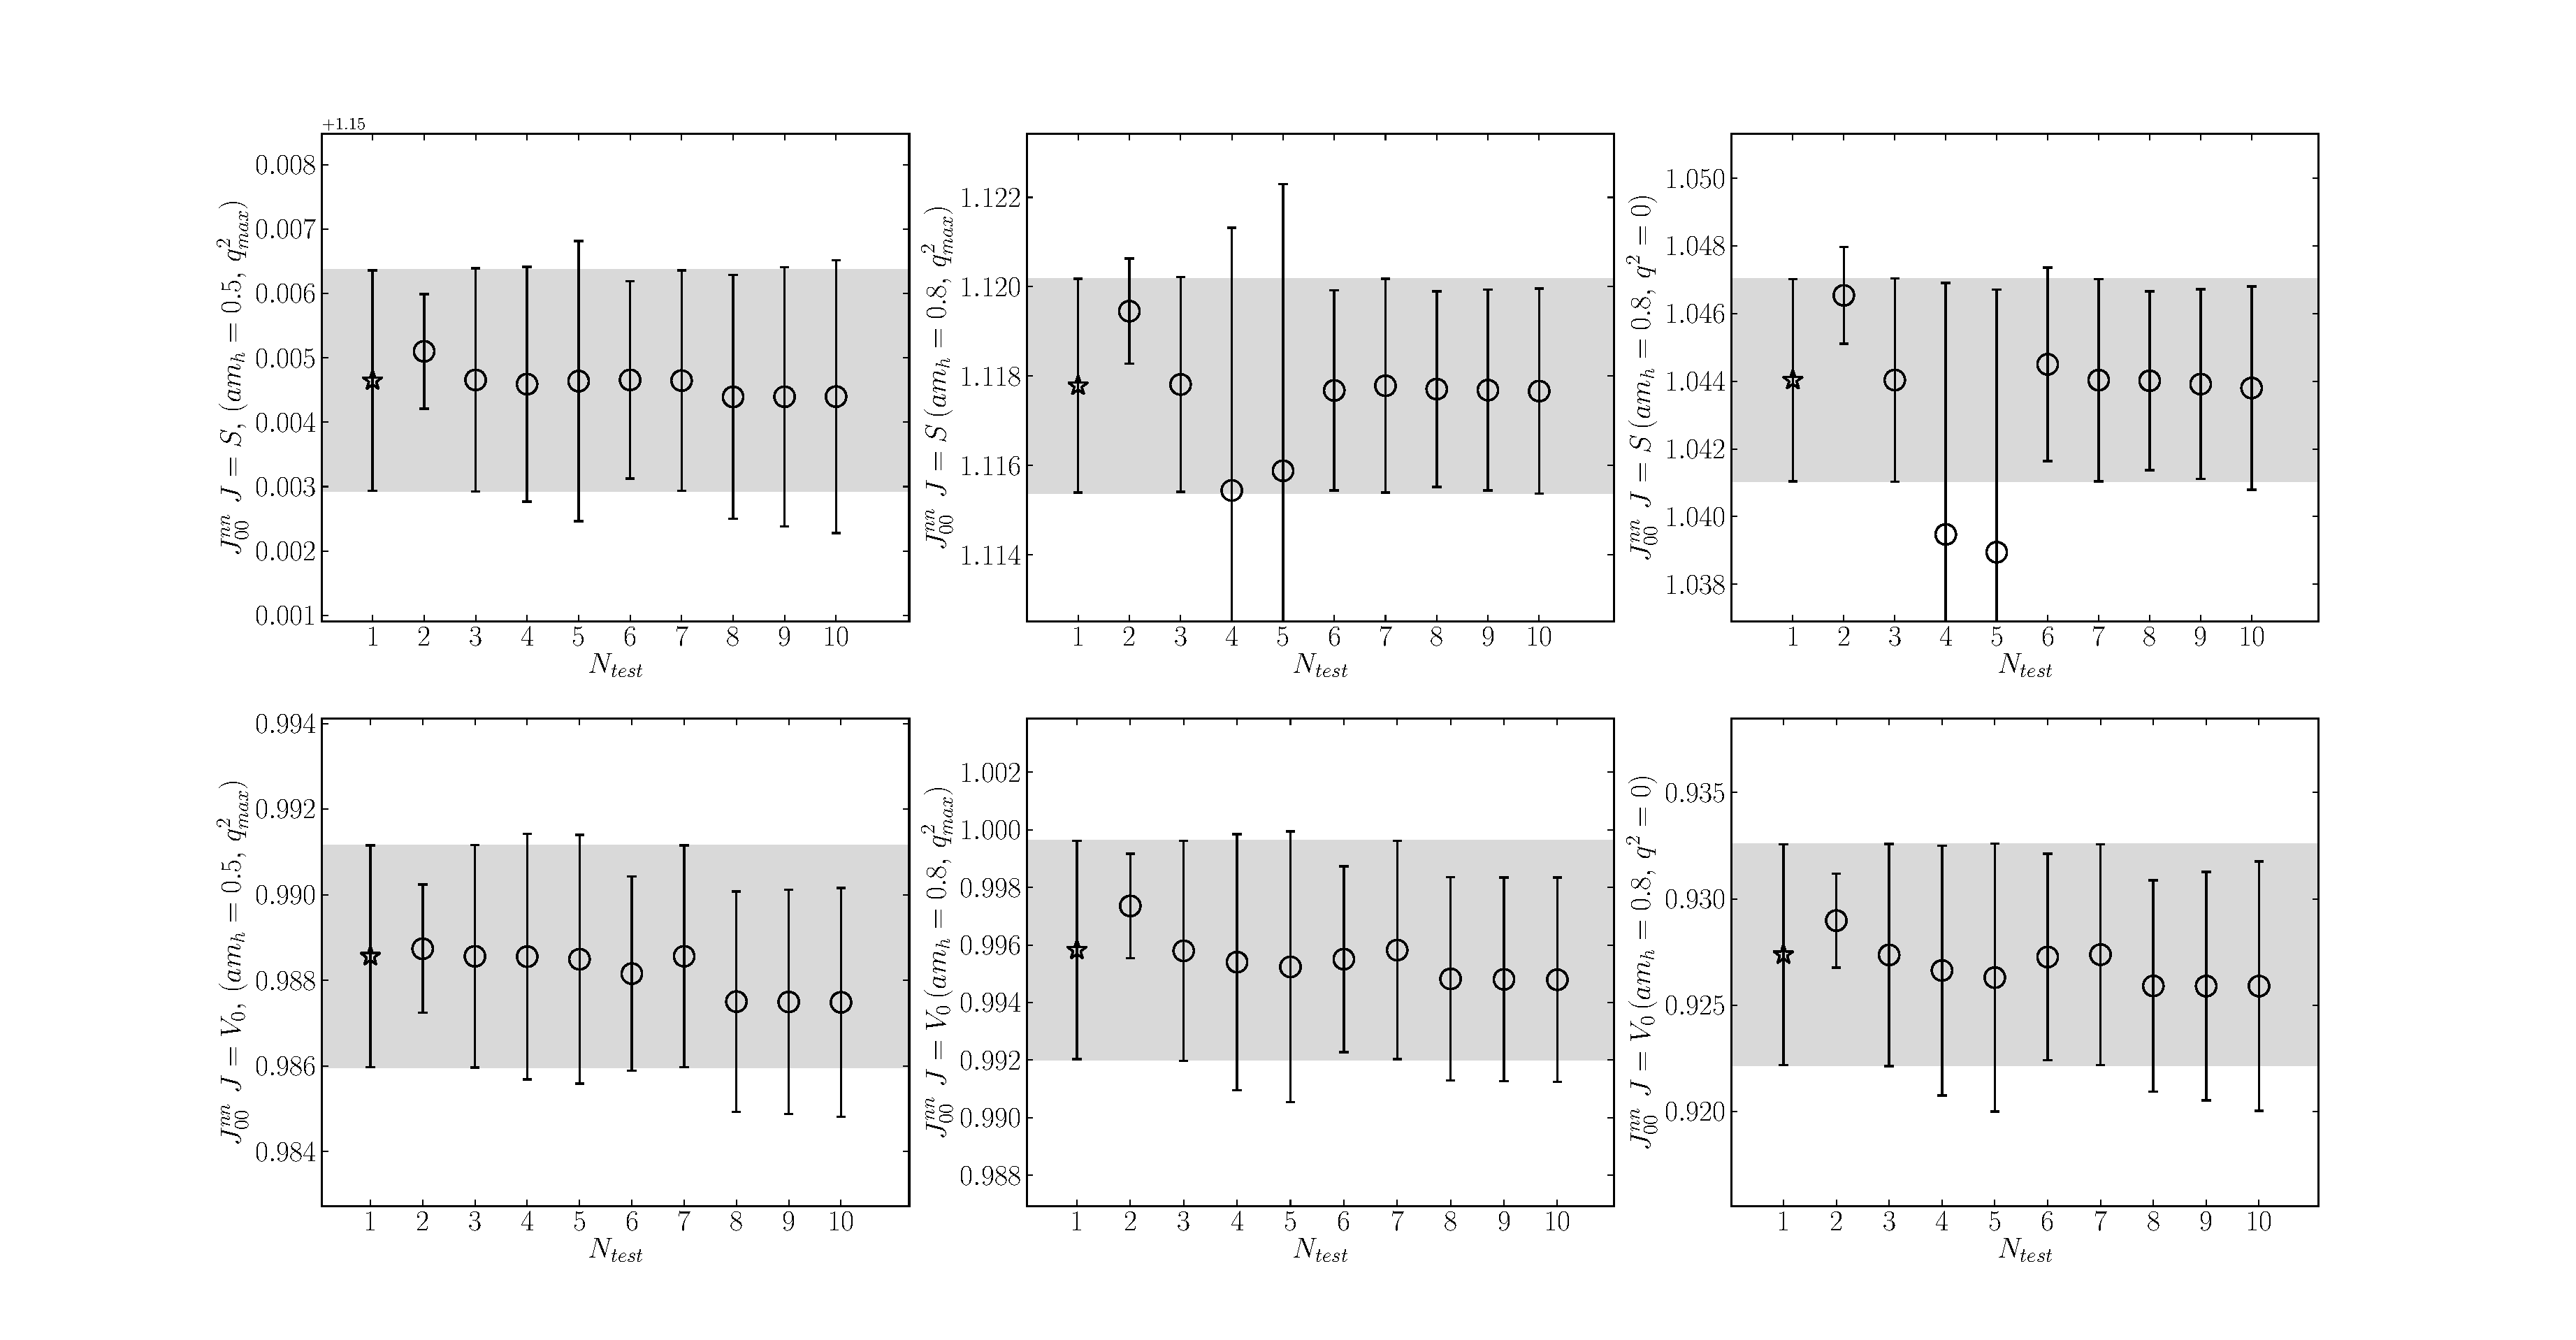
\includegraphics[width=1.4\textwidth]{images/BsDs/finecorr_fittest.pdf}
    \caption{Tests on the correlator fits on the fine ensemble. $N_{\text{test}}=1$ gives the final accepted result. $N_{\text{test}}=2$ and $3$ gives the results of setting $N_{\text{exp}}=4$ and $6$ respectively. $N_{\text{test}}=4$ gives the results when all priors are loosened by 50\%. $N_{\text{test}}=5$ gives the result of setting $t_{\text{cut}}=4$ rather than $2$ for all correlators. $N_{\text{test}}=6$ gives the result without marginalising out the $n=5$ excited state. $N_{\text{test}}=7$ gives the result of moving the svd cut from $10^{-3}$ to $10^{-2}$. $N_{\text{test}}=8,9,10$ gives the result of using a chained fit described above with priors for the full correlated fit given additional fractional errors of 100\%, 150\% and 200\% respectively. \label{fig:corr_tests_BsDs}}
\end{figure}

The stability issue is likely due to the size of the covariance matrix for the data, which must be inverted to estimate $\chi^2$. We took two steps toward mitigating this. The first is to impose an svd-cut. The second step we took was to employ a chained-fitting approach (this was required on the superfine and ultrafine data only). We first performed an array of smaller 'individual' fits, each fitting the correlators relevant only to one $m_h$ and one $|a{\bf{p}}_{D_s}|$ value. In the case of set 4, for example, this results in 11 separate fits. Then, a full simultaneous fit of all of the correlators was carried out, with priors set to the results of the smaller fits. To be conservative we multiplied these priors by $1\pm 1.5$, i.e., the priors end up with over 150\% variance. This both speeds up the full fit and improves the stability of the results. We tested the validity of the results by varying the additional fractional error between 100\% and 200\%, this caused negligible changes in the results. Since we did not need to take this measure on the fine ensemble, we performed both a standard simultaneous fit and chained fits of this type as a check for the chained fits. Tests 8, 9 and 10 on Fig. \ref{fig:corr_tests_BsDs} show the results of these chained fits in comparison to the more traditional fit.

The priors for the 'traditional' fits to fine and fine-physical (sets 2 and 3) data, and individual chained superfine and ultrafine (sets 4 and 5) fits, were set up as follows. We set Gaussian priors for the parameters $J_{jk}$, and log-normal priors for all other parameters. Using log-normal distributions forbids ground state energies $E_0^M$, excited energy differences $E_n^M-E_{n-1}^M$, and amplitudes $a_n^M$ from both becoming negative and moving arbitrarily close to zero, improving the stability of the fit.

Priors for ground state energies log($E_0^M$) and amplitudes log($a_0^M$) are set according to an empirical-Bayes approach, plots of effective energies and amplitudes of the correlation functions are inspected to deduce reasonable priors. The ground-state oscillating parameters log($a_0^{M,o}$), log($E_0^{M,o}$), are given the same priors as the non-oscillating states, with errors inflated by 50\%. The resulting priors always have a variance of at least 10 times that of the final result. The log of oscillating and non-oscillating excited state energies, log($E_i^{M,(o)}-E_{i-1}^{M,(0)}$), $i>0$ are given prior values of log($2\Lambda_{\text{QCD}}\pm \Lambda_{\text{QCD}}$). We set $\Lambda_{\text{QCD}}=0.5$GeV. The excited state amplitudes log($a_i^M$),$i>0$ are given priors of $-1.9\pm 3.3$ for non-oscillating states, and $-3.0\pm 2.0$ for oscillating states. The ground-state non-oscillating to non-oscillating 3-point parameter, $J_{00}^{nn}$ is given a prior of $1\pm 0.5$, and the rest of the 3-point parameters $J_{jk}^{nn}$ are given $0\pm 1$.

The current matrix elements we require can be extracted from the fit parameters via
\begin{align}
  \langle D_s| J | H_s \rangle |_{\text{lat}} = 2 \sqrt{M_{H_s}E_{D_s}} J^{nn}_{00}.
  \label{eq:currentfit}
\end{align}

\begin{figure}[htb!]
  \hspace{-30pt}
    \hspace{-10pt}
    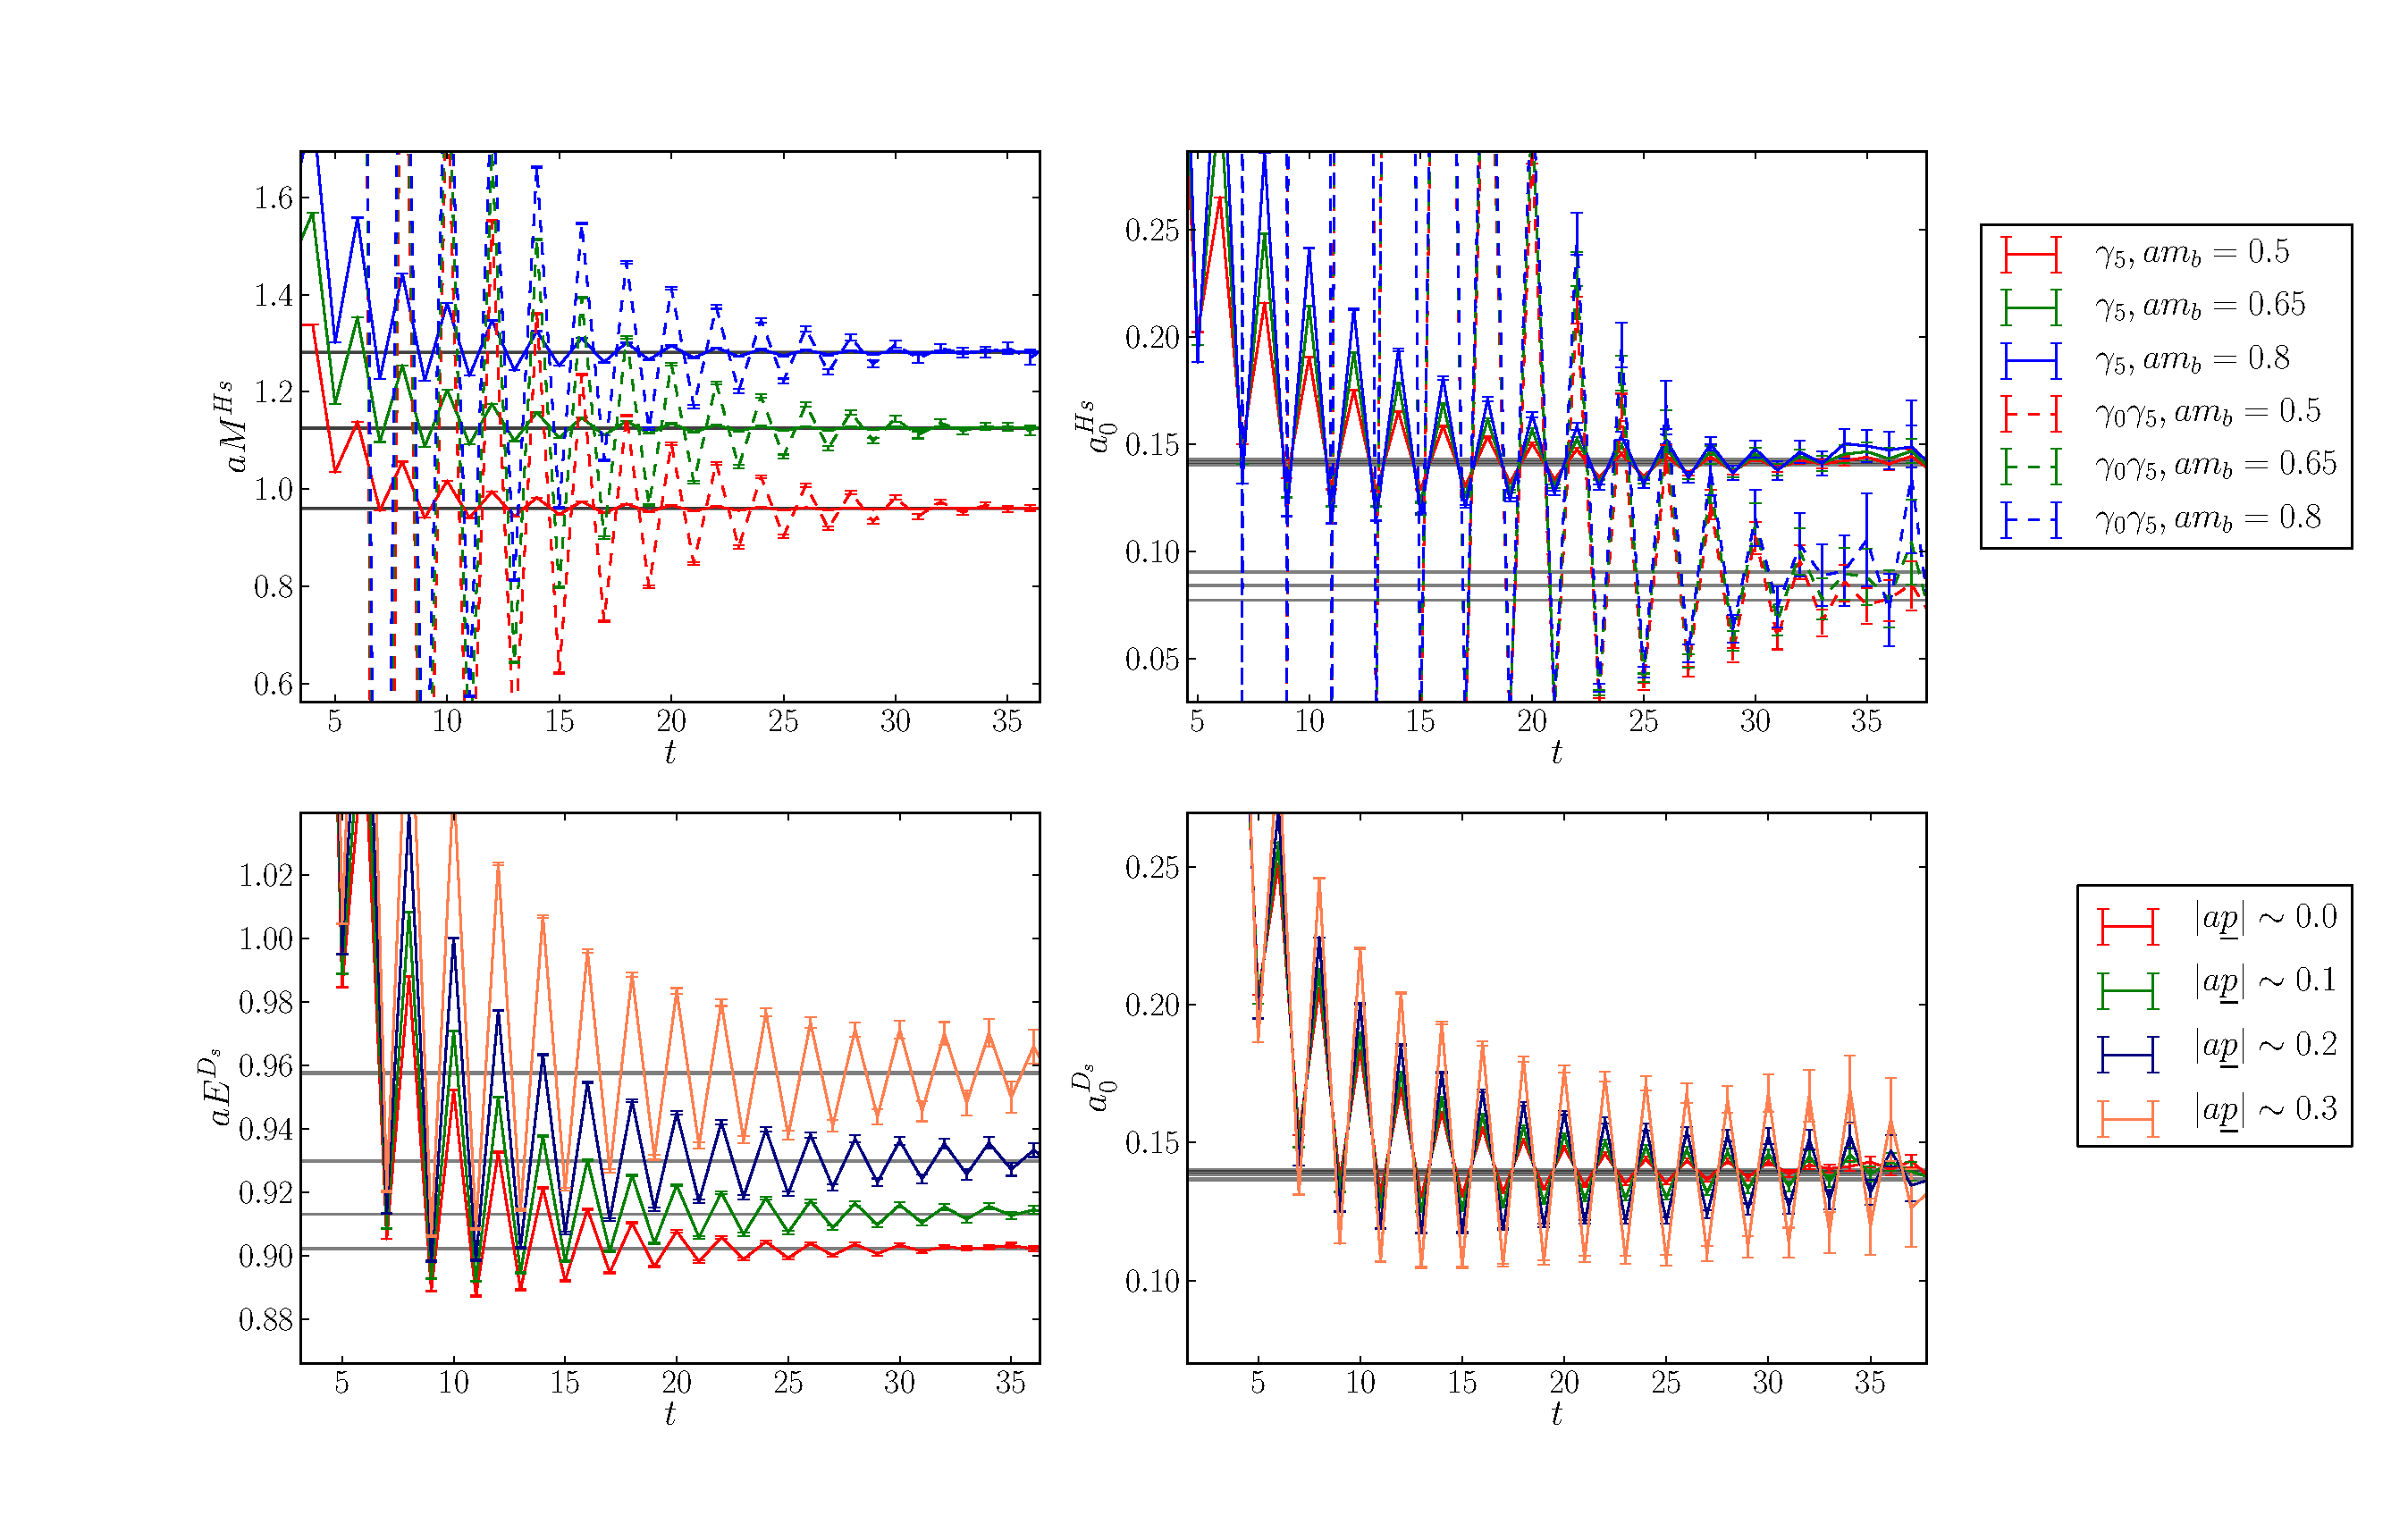
\includegraphics[width=1.2\textwidth]{images/BsDs/fine_2pt_summary.pdf}
    \caption{
Superaveraged effective energies (given by Eq. \eqref{eq:effectivemass}) and amplitudes (given by Eq. \eqref{eq:effectiveamp}) for a selection of 2-point correlators on the fine ensemble. The grey bands show the corresponding results for these quantities from the simultaneous Bayesian fits. These plots supply a further check of our correlator fits - results of the Bayesian fits are in good agreement with the effective energies and amplitudes.  \label{fig:2ptcorrs_BsDs}}
\end{figure}

\begin{figure}[htb!]
    \hspace{-60pt}
    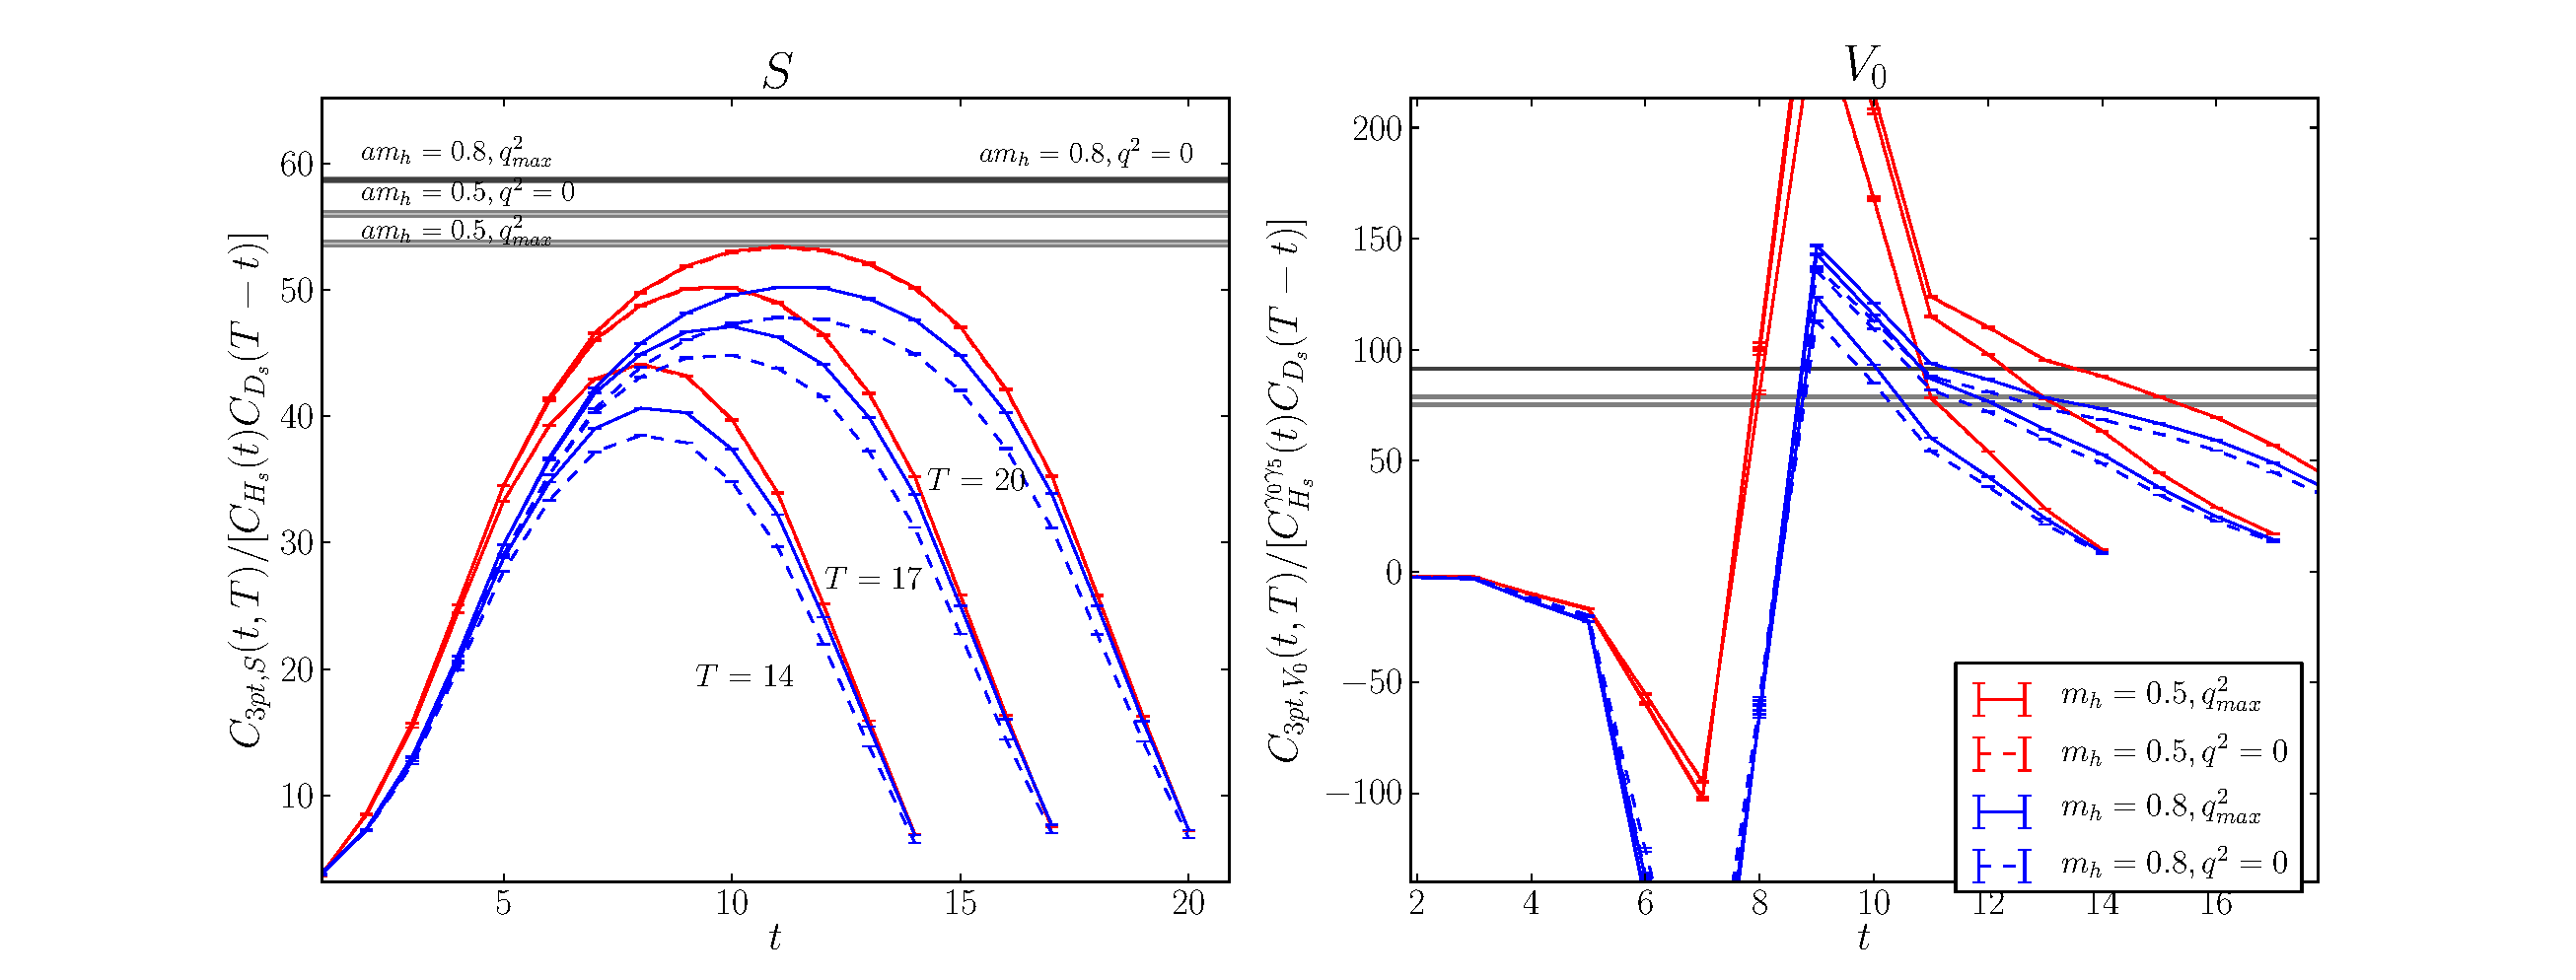
\includegraphics[width=1.3\textwidth]{images/BsDs/fine_3pt_summary.pdf}
    \caption{$\tilde{C}_3(t,T)/\tilde{C}^{H_s}(t) \tilde{C}^{D_s}(T-t)$, which should plateau at $J_{00}^{nn}$, in the fine ensemble for the $J=S$ and $J=V_0$ cases. The grey bands show the corresponding results for these quantities from the simultaneous Bayesian fits. Unfortunately, in the $V_0$ case the oscillating component dominates the correlation function, preventing any plateau from being visible. \label{fig:3ptcorrs_BsDs}}
\end{figure}

\subsection{Vector Current Renormalization}

In HISQ, the local scalar current $(1\otimes 1)$ (multiplied by the mass difference of flavours it is charged under) requires no renormalization due to its connection to the partially conserved vector current through the PCVC relation. This is not the case for the local temporal vector current $(\gamma_0\otimes \gamma_0)$. The partially conserved vector current is a complicated linear combination of many local and point-split lattice currents. In this calculation we use only the local part of the vector current, this improves the statistics of our results but creates the need for the resulting current matrix element to be multiplied by a matching factor $Z_V$ to produce the appropriate continuum current. We found $Z_V$ via a fully non-perturbative method \cite{Koponen:2013tua}.

When both meson states in the matrix elements are at rest (the zero recoil point), the scalar and local vector matrix elements are related via the PCVC relation:
\begin{align}
  ( M_{H_s}& - M_{D_s} ) Z_V \langle D_s | V_0 | \hat{H}_s \rangle|_{\text{lat}}(q^2_{\text{max}}) = (m^{\text{val}}_{h0} - m^{\text{val}}_{c0}) \langle D_s | S | H_s \rangle|_{\text{lat}}(q^2_{\text{max}}).
  \label{eq:ward}
\end{align}
$Z_V$ can be extracted from this relation since the matrix elements are already computed as part of the calculation. Our calculation is self-renormalizing, in the sense that the normalization can be found at no extra computational cost. The $Z_V$ values found on each ensemble and $am^{\text{val}}_{h0}$ are given in Table \ref{tab:norms}.

We also removed tree-level mass-dependent discretization effects using a normalization constant $Z_{\text{disc}}$ defined in Eq. \eqref{eq:Zdisc}.

Combining these normalizations with the lattice current from the correlation function fits, we found values for the form factors at a given heavy mass, lattice spacing, and $q^2$:
\begin{align}
  \nonumber
  f_0^s&(q^2) = {m^{\text{val}}_{h0} - m^{\text{val}}_{c0}\over M_{H_s}^2 - M_{D_s}^2 } Z_{\text{disc}} \langle D_s | S | H_s \rangle|_{\text{lat}}(q^2) \\
  \label{eq:normalizations}
  f_+^s&(q^2) = {Z_{\text{disc}} \over 2M_{H_s}} \times \\ \nonumber &{ \delta^M \langle D_s | S | B_s \rangle|_{\text{lat}}(q^2) - q^2 Z_V \langle D_s | V_0 | B_s \rangle|_{\text{lat}}(q^2) \over {\bf{p}}^2_{D_s}}.
\end{align}
I have here explicitly denoted the dependence of the matrix elements on $q^2$ as a reminder that the matrix elements have $q^2$ dependence via the $D_s$ momentum.

\begin{table}
\begin{center}
\begin{tabular}{ c c c c }
\hline
Set & $am_h^{\text{val}}$ & $Z_V$& $Z_{\text{disc}}$\\ [0.5ex]
\hline
0 & 0.5 & 1.0151(32) & 0.99819\\ [0.5ex] 
 & 0.65 & 1.0240(37) & 0.99635\\ [0.5ex] 
 & 0.8 & 1.0368(49) & 0.99305\\ [0.5ex] 
\hline
1 & 0.5 & 1.0134(24) & 0.99829\\ [0.5ex] 
 & 0.8 & 1.0348(29) & 0.99315\\ [0.5ex] 
\hline
2 & 0.427 & 1.0027(25) & 0.99931\\ [0.5ex] 
 & 0.525 & 1.0059(29) & 0.99859\\ [0.5ex] 
 & 0.65 & 1.0108(37) & 0.99697\\ [0.5ex] 
 & 0.8 & 1.0197(49) & 0.99367\\ [0.5ex] 
\hline
3 & 0.5 & 1.0037(40) & 0.99889\\ [0.5ex] 
 & 0.65 & 1.0087(46) & 0.99704\\ [0.5ex] 
 & 0.8 & 1.0160(53) & 0.99375\\ [0.5ex] 
\hline
\end{tabular}
    \caption{Normalization constants applied to the lattice axial vector current in \eqref{eq:normalizations}. $Z_V$ is found from \eqref{eq:ward} and $Z_{\text{disc}}$ from \eqref{eq:Zdisc}. \label{tab:norms}}
\end{center}
\end{table}

\subsection{Extrapolation to the Physical Point}
\label{sec:extrapolation}

I will now address the extrapolation of the $f_{0}^s(q^2)$ and $f_{+}^s(q^2)$ values to continuum, physical quark masses and arbitrary $q^2$. We took two complementary approaches to the extrapolation.

One we refer to as the {\textit{ratio}} approach, in which one extrapolates the quantity
\begin{align}
  R^s_{0,+}(q^2) \equiv {f^s_{0,+}(q^2)\over f_{H_c}\sqrt{M_{H_c}}}\,.
  \label{eq:ratio}
\end{align}
to the physical point. Discretisation effects appear to cancel to a large extent in this ratio, resulting in a better controlled continuum extrapolation. The value at the physical point is then multiplied by $f_{B_c}\sqrt{M_{B_c}}$ to isolate the form factors, where we find $f_{B_c}$ via a separate extrapolation (detailed in Sec. \ref{sec:stability_BsDsstar}), and take the PDG value for $M_{B_c}$ \cite{PhysRevD.98.030001}. While this approach improves the continuum extrapolation, it has the downside of introducing errors from scale-setting on account of $R_{0,+}^s(q^2)$ being dimensionful quantities (as opposed to $f^s_{0,+}(q^2)$ which are dimensionless).

In the other method, that we refer to as the {\textit{direct}} approach, one simply extrapolates the form factors to the physical point. The form factors by themselves have larger discretisation effects than $R_{0,+}^s(q^2)$, but since $f^s_{0,+}$ are dimensionless, the results are completely insensitive to scale-setting uncertainty.

We use identical fit functions for both approaches. In the below discussion, we use the notation $F^s_{0,+}(q^2)$ to denote either $f^s_{0,+}(q^2)$ or $R_{0,+}^s(q^2)$, depending on the approach being applied.

\subsubsection{Kinematic Behaviour}

Our fit form for the extrapolation is a modified version of the Bourrely-Caprini-Lellouch (BCL) parameterization for pseudoscalar$\to$pseudoscalar form factors \cite{Bourrely:2008za}:
\begin{align}
  \label{eq:BCL}
  &F^s_0(q^2)|_{\text{fit}} = {1\over 1 - {q^2\over M_{H_c^0}^2} } \sum_{n=0}^{N-1} a_n^0 z^n(q^2), \\
  &F^s_+(q^2)|_{\text{fit}} = {1\over 1 - {q^2\over M_{H_c^*}^2} } \sum_{n=0}^{N-1} a_n^+ \left( z^n(q^2) - {n\over N} (-1)^{n-N} z^N(q^2) \right). \nonumber
\end{align}
The functon $z(q^2)$ maps $q^2$ to a small region inside the unit circle on the complex plane, defined by
\begin{align}
  z(q^2) = {\sqrt{t_+ - q^2} - \sqrt{t_+ - t_0} \over \sqrt{t_+ - q^2} + \sqrt{t_+ - t_0} },
\end{align}
where $t_+ = (M_{H_s}+M_{D_s})^2$, and we chose $t_0$ to be $t_0 = 0$. This $t_0$ choice means that at $q^2=0$ the fit functions simplify to $F_{0,+}^s(0) = a_0^{0,+}$. Throughout the physical range of $q^2$, $z$ is restricted to the range $0<z<0.06$, resulting in a fast converging series in powers of $z$. We truncate at $N=3$, adding further orders of $z^n$ does not affect the results of the fit.

The factors in front of the sums in the BCL parameterization account for subthreshold poles in the form factors due to the production of on-shell $H_{c0}$ and $H_c^*$ states in the crossed channel of the semileptonic decay.

To estimate $M_{H_{c0}}$, the scalar heavy-charm meson mass, at each of the heavy masses we used, we leveraged the fact that the splitting $\Delta_0 = M_{H_{c0}} - M_{H_c}$ is due to an orbital excitation and therefore independent of the heavy quark mass. This has been calculated in \cite{Dowdall:2012ab} to be $\Delta_0 = 0.429(13)$GeV. Combined with an $H_c$ mass from our correlators, we can construct the $H_{c0}$ mass: $M_{H_{c0}} = M_{H_c} + \Delta_0$. We did not take the error on $\Delta_0$ into account in the fit since the precise position of the pole has a small effect on the fit results.

To estimate $M_{H^*_c}$, the vector heavy-charm mass, we use the fact that the splitting $ M_{H_c^*} - M_{H_c}$ vanishes in the infinite heavy mass limit. $M_{H_c^*}$ then takes the approximate form $M_{H_c^*} \simeq M_{H_c} + \order{1/m_h}$. To reproduce this behaviour we use the ansatz $M_{H_c^*} = M_{H_c} + x/M_{\eta_h}$, and fix $x$ at the physical point to find $x=0.508$GeV$^2$. To do this we used the result $M_{B_c^*}-M_{B_c}=54(3)\,$MeV from \cite{Dowdall:2012ab}.

\subsubsection{Heavy Mass and Discretisation Effects}

To account for variation in heavy mass and discretisation effects in a general way, we gave the following form to each of the $a_n^{0,+}$ coefficients:
\begin{align}
  \nonumber  a_n^{0,+} = & \,\,\left( 1 + \rho^{0,+}_n \text{log}\left(M_{\eta_c}\over M_{\eta_h}\right)\right) \times \\ \nonumber
  &\sum_{i,j,k = 0}^{2,2,2} d^{0,+}_{ijkn} \left({2\Lambda_{\text{QCD}}\over M_{\eta_h} }\right)^{i} \left({ am^{\text{val}}_{h0} \over \pi }\right)^{2j} \left({ aE_{D_s} \over \pi }\right)^{2k} \\ &\times\left(1 + \mathcal{N}_{\text{mistuning},n}^{0,+} \right)\,.
      \label{eq:mhfitfun}
\end{align}

To understand this form, focus first on the sum. Powers of $(2\Lambda_{\text{QCD}}/M_{\eta_h})$ give an HQET inspired way of quantifying the variation in the results due to the changing heavy mass. $M_{\eta_h}$ varies strongly and monotonically with the heavy quark mass, so acts as a suitable proxy. $\Lambda_{\text{QCD}}$ is the confinement scale, which we set to 0.5GeV.

The two scales expected to be the largest sources of discretisation effects are the heavy mass $am_{h0}^{\text{val}}$, and the energy in the $D_s$ meson, $aE_{D_s}$, especially when it is given a large spatial momentum. Adding further, smaller scales, like $a\Lambda_{\text{QCD}}$, had no effect on the results.

The coefficients $d^{0,+}_{ijkn}$ are fit parameters given prior distributions of $0\pm 2$. In the ratio case, these carry mass dimension GeV$^{-3/2}$, hence this prior corresponds to a prior of $0\pm (2\Lambda_{\text{QCD}})^{-3/2}$.

To account for any required matching between HQET and QCD, we included a log term in front of the sum. $\rho^{0,+}_n$ are fit parameters with prior distribution $0\pm 1$.

The fact that $f^s_+(0) = f^s_0(0) \,(\,\Rightarrow a^+_0 = a^0_0)$ is a very powerful constraint within the heavy-HISQ approach. Since this must be true at all $m_h$, this translates to constraints in the fit parameters: $d^+_{i000}=d^0_{i000} \,\forall \,i$ and $\rho^+_0 = \rho^0_0$. We imposed these constraints in the fit, which serve to stablize the extrapolation in the heavy mass direction.

\subsubsection{Mass Mistunings}

We dealt with possible mistuning in the $c$, $s$ and $l$ masses in the same way as in the $B_s\to D_s^*$ study. We included the terms $\mathcal{N}_{\text{mistuning},n}^{0,+}$ in each $a^{0,+}_n$ coefficient, given by
\begin{align}
  \mathcal{N}_{\text{mistuning},n} &= {c_{s,n}^{\text{val}} \delta^{\text{val}}_s + c_{s,n} \delta_s + 2 c_{l,n} \delta_l \over 10 m_s^{\text{tuned}} }
    \label{eq:mistuning}
  +c_{c,n}^{0,+} \left({ M_{\eta_c} - M_{\eta_c}^{\text{phys}} \over M_{\eta_c}^{\text{phys}}}\right)\,,
\end{align}
where $c^{0,+}_{l,n}$, $c^{0,+}_s$ and $c^{0,+}_{ci}$ are fit parameters with prior distributions $0\pm 1$. $\delta_{s,l}^{(\text{val})}$ are defined in Sec. \ref{sec:mistuning_BsDsstar} and $m_s^{\text{tuned}}$ is defined in Eq. \eqref{eq:strange_mistuning}.

%% The strange mistuning is accounted for here using an approach first used in \cite{Chakraborty:2014aca}. We define the term $\delta_s = m^{\text{val}}_{s0} - m_s^{\text{tuned}}$, where $m_s^{\text{tuned}}$ is defined by
%% \begin{align}
%%   m_s^{\text{tuned}} = m^{\text{val}}_{s0} \left({ M^{\text{phys}}_{\eta_s} \over M_{\eta_s} }\right)^2.
%% \end{align}
%% $M_{\eta_s}^{\text{phys}}$ was determined in a lattice simulation from the masses of the pion and kaon \cite{Dowdall:2013rya}.

%% We similarly account for (sea) light quark mistuning by defining $\delta_l = m_{l0} - m_l^{\text{tuned}}$. We find $m_l^{\text{tuned}}$ from $m_s^{\text{tuned}}$, using the fact that the ratio of quark masses is regularization independent, and was calculated in \cite{Bazavov:2014wgs}:
%% \begin{align}
%%   \left.\frac{m_s}{m_l}\right\rvert_{\textrm{phys}} = 27.18(10).
%% \end{align}
%% We set $m_l^{\text{tuned}}$ to $m_s^{\text{tuned}}$ divided by this ratio.

All higher order contributions, like $\delta^{(\text{val})\,2}_{s,l}$ or $(M_{\eta_c}-M_{\eta_c}^{\text{phys}})^2$ are too small to be resolved by our lattice data, so are not included in the fit.

\subsubsection{Negligable Effects}

Finite volume effects are negligible in our calculation, we do not include any associated error. Finite volume corrections to the $B\to Dl\nu$ form factors in chiral perturbation theory were calculated in \cite{Laiho:2005ue}. They found the $B\to Dl\nu$ form factor at zero recoil, with a lattice size of $L=2.5$fm, and pion mass equal to or greater than physical, never exceeded $10^{-4}$. There is no reason to believe changing the spectator quark from light to strange, and moving away from zero recoil, will increase this effect.

In our simulation we set $m_u=m_d\equiv m_l$, this means our results do not account for isospin breaking. By moving the $m_l^{\text{tuned}}$ value up and down by the PDG value for $m_d-m_u$, we tested for any signs of isospin breaking having an effect on the results. The resulting effect was negligible in comparison to all other sources of error.

Since we take the physical result at $M_{\eta_h}=M_{\eta_b}$, the uncertainty in $M_{\eta_b}$ will contribute an uncertainty in the final result. We used the PDG result for $M_{\eta_h}$ \cite{PhysRevD.98.030001}. However, $\bar{b}-b$ annihilation and electroweak corrections make this somewhat different to the appropriate value on the lattice. We estimated the corresponding uncertainty in $M_{\eta_b}$ to be no greater than $\pm10$MeV. To see how this changes the result of the extrapolation, we varied $M_{\eta_b}$ up and down by 10MeV and studied how our result at $f_0(q^2_{\text{max}})$ changes. The change is never greater than $10^{-4}$, which is negligible in comparison to the other errors.

\section{Results}
\label{sec:results}

Tables \ref{tab:masses} and \ref{tab:kinetic} in Sec. \ref{sec:tables} give numerical values for the form factors, the ratios $R_{0,+}^s(q^2)$, and parameters extracted from the correlation function fits required for the extrapolations to the physical point.

I will first show results from the ratio method, then the direct method. In both cases, we performed a simpler fit at zero recoil first, then a larger fit taking into account all data throughout $q^2$.  In each case, our results are statistics dominated. The results from the two methods are in good agreement.

\subsection{Ratio Method}
\label{sec:ratiomethod}

\subsubsection{Zero Recoil}

\begin{figure}[htb!]
  \begin{center}
  \hspace{-10pt}
  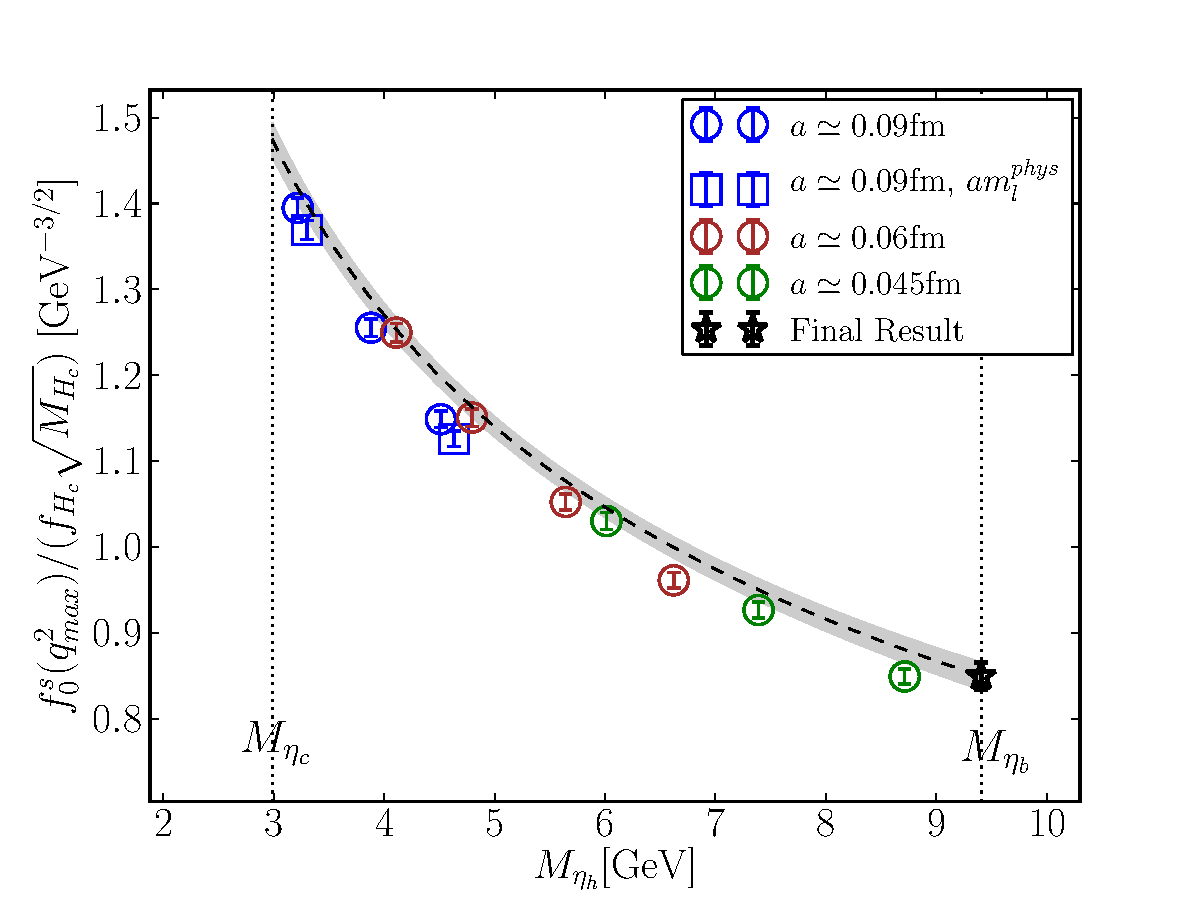
\includegraphics[width=0.85\textwidth]{images/BsDs/ratio/f0fHc_vsmh.pdf}
  \caption{ $R_0^s(q^2_{\text{max}}) = f_0^s(q^2_{\text{max}})/(f_{H_c}\sqrt{M_{H_c}})$ against $M_{\eta_h}$ (a proxy for the heavy quark mass). The grey band shows the result of the extrapolation at $a=0$ and physical $l$,$s$ and $c$ masses. Sets listed in the legend follow the order of sets in table \ref{tab:ensembles}. \label{fig:ratioq2max}}
    \end{center}
\end{figure}

We performed an isolated extrapolation of $R^s_0(q^2_{\text{max}})$ to the physical point. To do this we used a simplified fit form for $R^s_0(q^2_{\text{max}})$ consisting of the right hand side of \eqref{eq:mhfitfun},with the index $n$ discarded.
We find
\begin{align}
  R_0^s(q^2_{\text{max}}) = {f_0^s(q^2_{\text{max}})\over f_{B_c}\sqrt{M_{B_c}}} = 0.843(18) \text{GeV}^{-3/2}\,.
\end{align}
The extrapolation against $M_{\eta_h}$ is illustrated in Fig. \ref{fig:ratioq2max}. As can be seen here, data for this ratio has a very weak dependence on the lattice spacing. The error budget for this result is given in Table \ref{ratioq2max_budget}.

\begin{table}[htb!]
  \begin{center}
    \begin{tabular}{c c}
      \hline
      Source & \% Fractional Error \\ [0.5ex]
      \hline
      Statistics & 1.72  \\ [1ex]
      Scale Setting & 1.35  \\ [1ex]
      $m_h \to m_b$, & 0.87  \\ [1ex]
      $a\to 0$ & 0.16  \\ [1ex]
      mistuning & 0.72 \\ [1ex]
      \hline
      Total & 2.16 \\ [1ex]
      \hline
    \end{tabular}
  \end{center}
  \caption{Error budget for $R_0^s(q^2_{\text{max}})$. \label{ratioq2max_budget}}
\end{table}

We performed a number of tests on this zero recoil extrapolation to test the stability of our fit form, results are given in Fig. \ref{fig:ratiotests}.

\begin{figure}[htb!]
  \begin{center}
  \hspace{-20pt}
  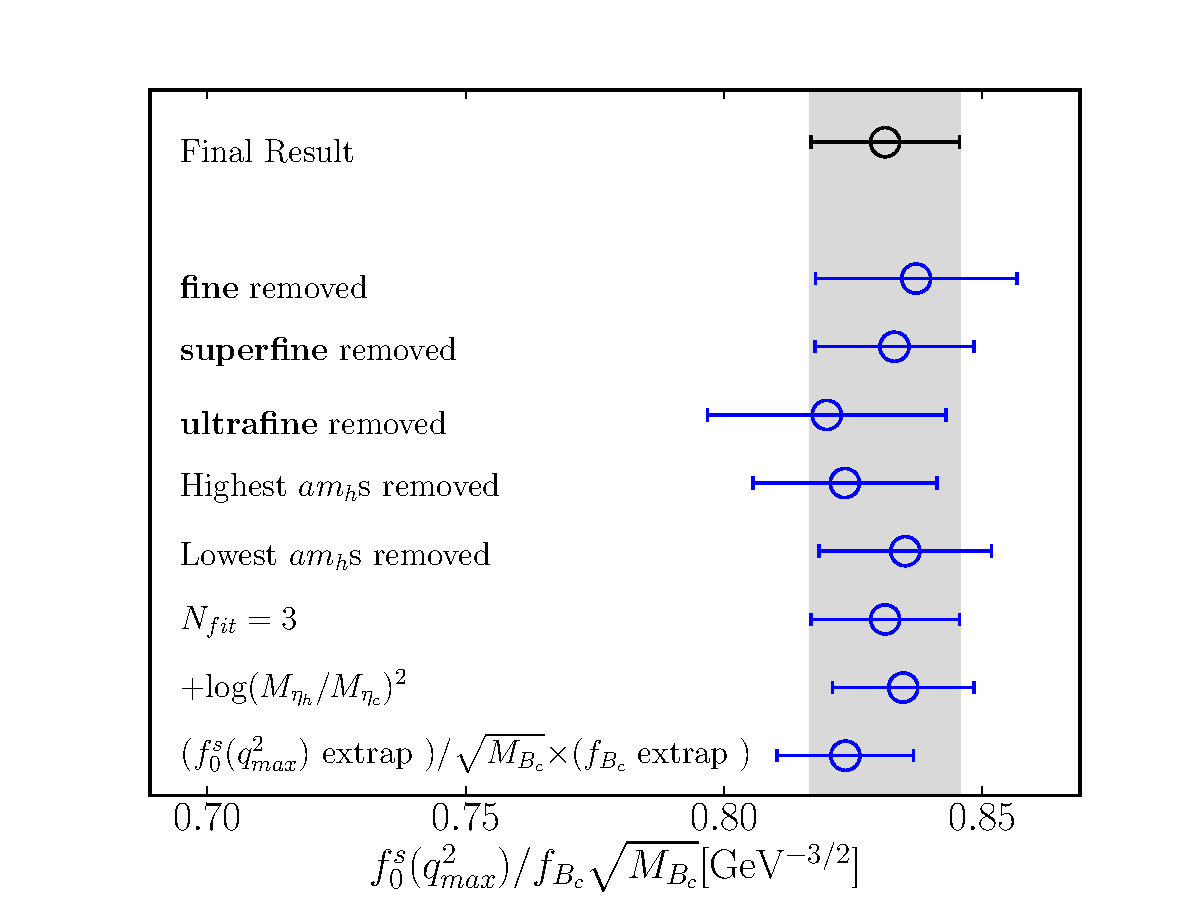
\includegraphics[width=0.85\textwidth]{images/BsDs/ratio/f0dcq2max_stability.pdf}
  \caption{ Results of tests of the $R_0^s(q^2_{\text{max}})$ extrapolation. The top three blue points show $R_0^s(q^2_{\text{max}})$ at continuum and physical quark mass, if data from the fine, superfine or ultrafine ensembles are not used in the fit. The fourth and fifth blue points show the result if data at the highest/lowest $am_{h0}^{\text{val}}$ value on each ensemble are removed. The point labelled $N_{fit}=3$ is the result of extending the sum in \eqref{eq:mhfitfun} such that it truncates at 3 rather than 2 in each of the $i,j,k$ directions. The point labelled $+\text{log}(M_{\eta_h}/M_{\eta_c})^2$ represents the result of adding a $\rho_{2,\,n} \text{log}(M_{\eta_h}/M_{\eta_c})^2$ term in the first set of brackets in \eqref{eq:mhfitfun}, where $\rho_{2,\,n}$ are new fit parameters with the same prior distributions as $\rho_{n}$. Similarly $+\text{log}(M_{\eta_h}/M_{\eta_c})/M_{\eta_h}$ shows the result of adding this term multiplied by $\rho_{2,\,n}$. The lowest point shows the result of our direct extrapolation of $f_0^s(q^2_{\text{max}})$ to the physical point, divided by the PDG value for $\sqrt{M_{B_c}}$ \cite{PhysRevD.98.030001} and the result of our extrapolation of $f_{B_c}$ to the physical point detailed in Sec. \ref{sec:stability_BsDsstar}.
    \label{fig:ratiotests}}
  \end{center}
\end{figure}

\subsubsection{Non-zero Recoil}

\begin{figure}[htb!]
  \hspace{-85pt}
  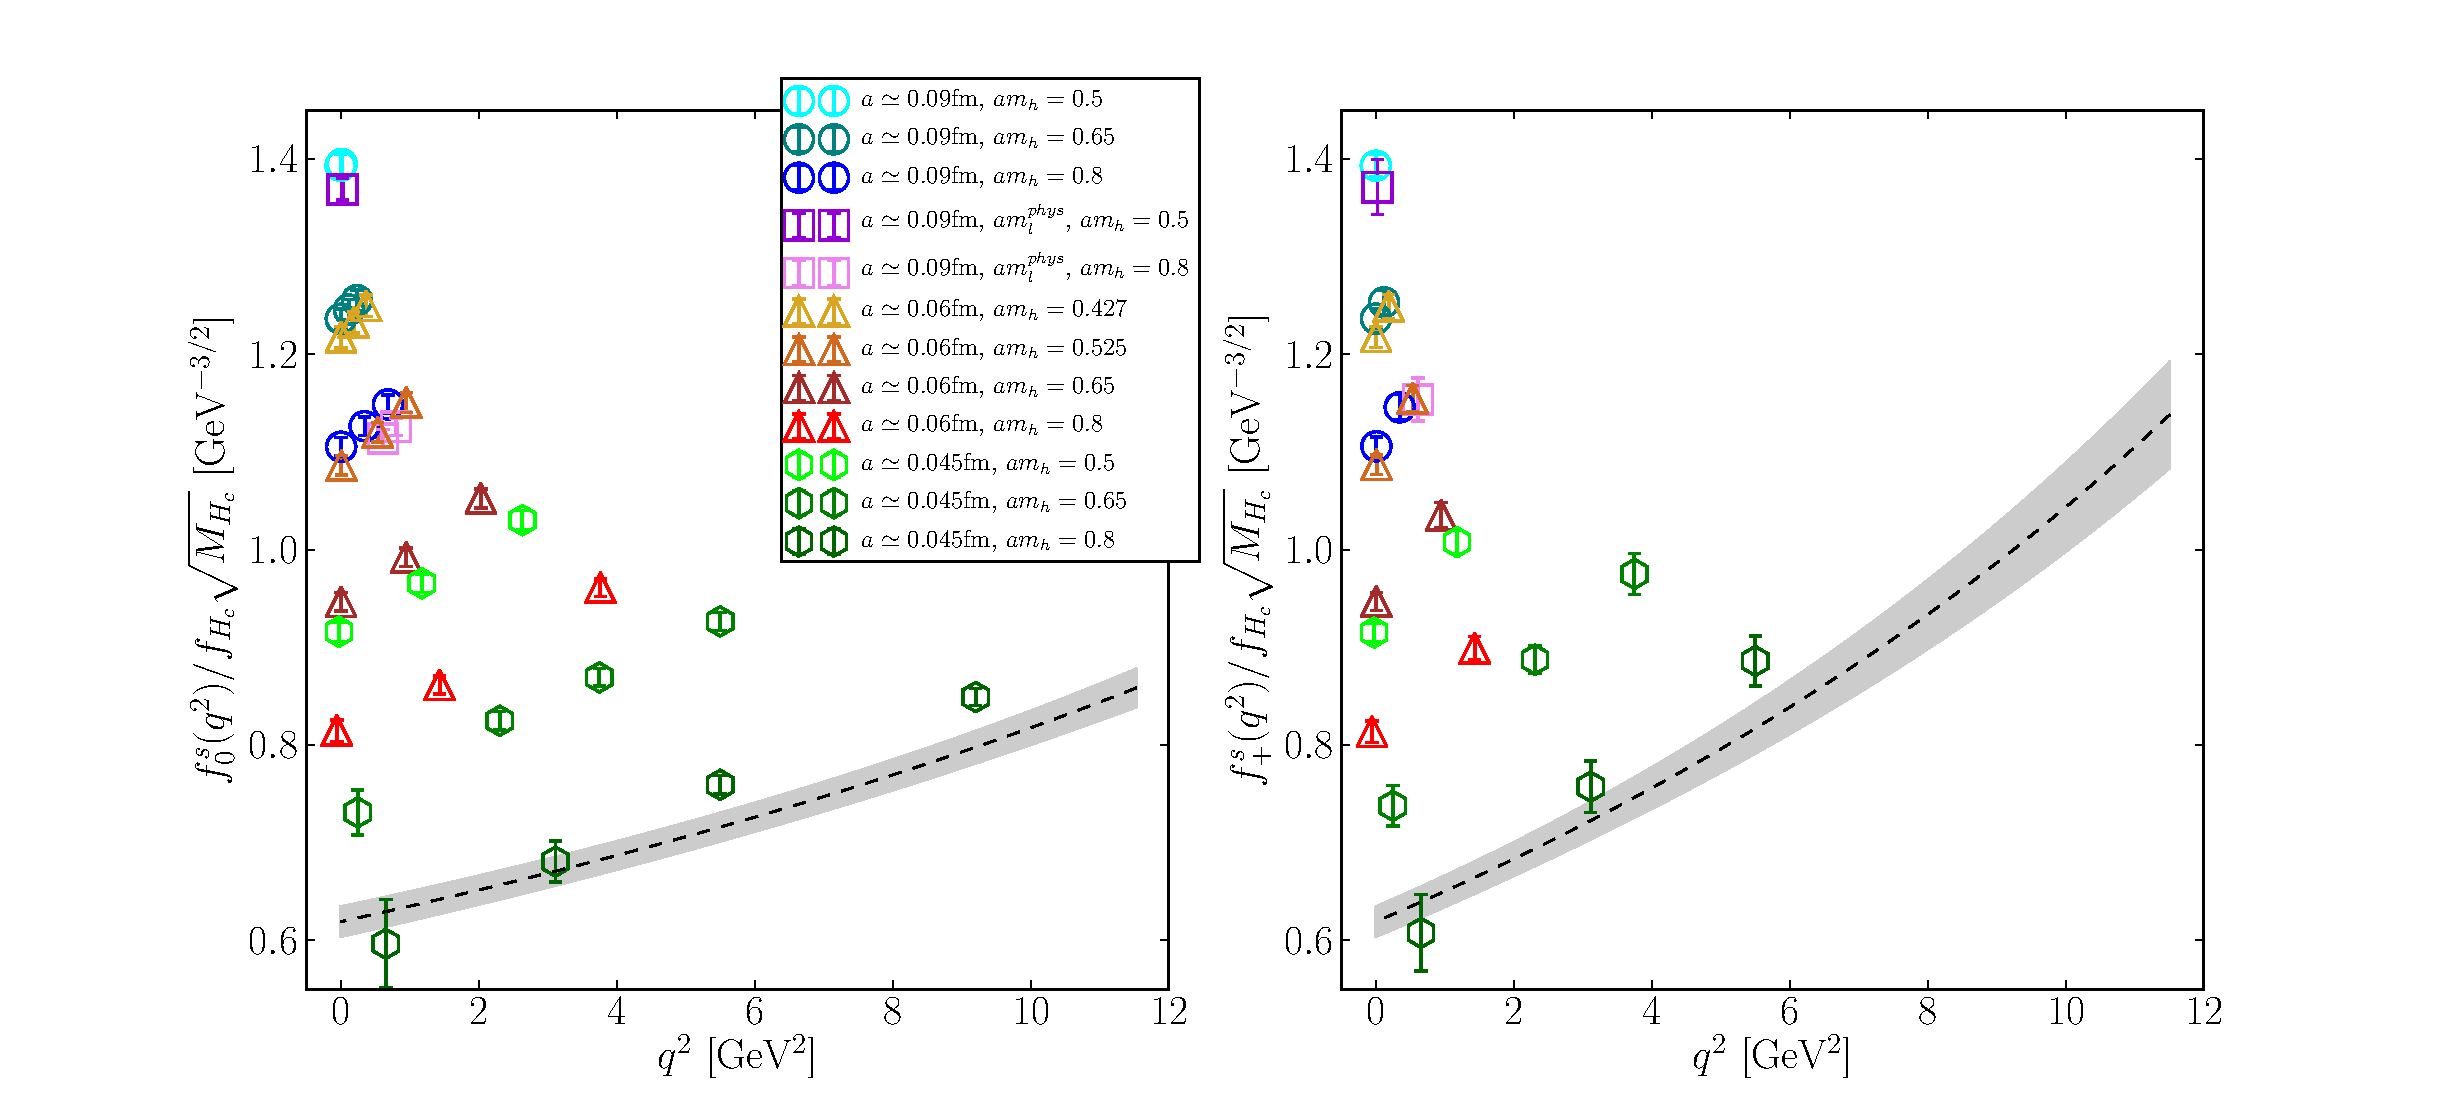
\includegraphics[width=1.50\textwidth]{images/BsDs/ratio/f0fpfHc_vsq2.pdf}
  \caption{ $R_{0,+}^s(q^2) = f_{0,+}^s(q^2)/(f_{H_c}\sqrt{M_{H_c}})$ against $q^2$. The grey band shows the result of the extrapolation at $a=0$ and physical quark masses. Sets listed in the legend follow the order of sets in table \ref{tab:ensembles}. \label{fig:ratiodata}}
\end{figure}

Fig. \ref{fig:ratiodata} shows the result of the full extrapolation of $R_{0,+}^s(q^2)$ throughout the $q^2$ range described in Sec. \ref{sec:extrapolation}. As the heavy mass increases, the $q^2$ range, $0 < (M_{H_s}-M_{D_s})^2$ expands.

To isolate the form factors, the resulting functions $R_{0,+}^s(q^2)$ were multiplied by $\sqrt{M_{B_c}}$ (using the PDG value) and $f_{B_c}$ from our determination detailed in Sec. \ref{sec:stability_BsDsstar}. The resulting form factors are shown in Fig. \ref{fig:ratiovsdirect}, against the form factors found via the direct method.

\subsection{Direct Method}

\subsubsection{Zero Recoil}
\label{sec:directq2max}

\begin{figure}[htb!]
  \begin{center}
  \hspace{-10pt}
  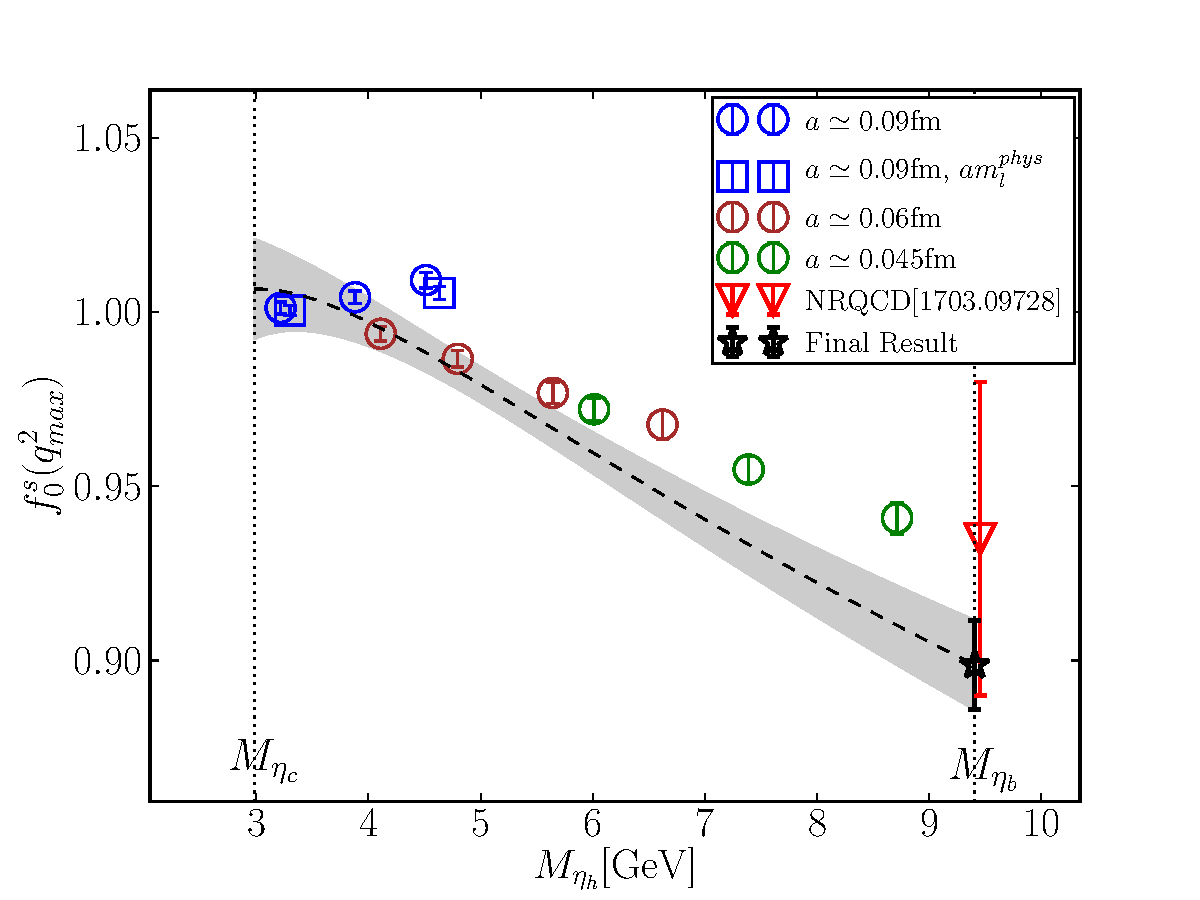
\includegraphics[width=0.85\textwidth]{images/BsDs/direct/f0q2max_vsmh.pdf}
  \caption{ $f_0^s(q^2_{\text{max}})$ against $M_{\eta_h}$ (a proxy for the heavy quark mass). The grey band shows the result of the extrapolation at $a=0$ and physical quark masses. We also include the result from a previous lattice calculation, which used the NRQCD discretisation for the $b$ quark \cite{Monahan:2017uby}. Sets listed in the legend follow the order of sets in Table \ref{tab:ensembles}. \label{fig:directq2max}}
  \end{center}
\end{figure}

We performed an isolated extrapolation of $f^s_0(q^2_{\text{max}})$ to the physical point. Once again, this was performed using a fit function for $f^s_0(q^2_{\text{max}})$ consisting of the right hand side of Eq. \eqref{eq:mhfitfun} with the index $n$ discarded. We find
\begin{align}
  f_0^s(q^2_{\text{max}}) = 0.899(13).
  \label{eq:f0s_direct}
\end{align}
The extrapolation against $M_{\eta_h}$ is shown in Fig. \ref{fig:directq2max}. The error budget for this result is given in Table \ref{directq2max_budget}.

\begin{table}[htb!]
  \begin{center}
    \begin{tabular}{c c}
      \hline
      Source & \% Fractional Error \\ [0.5ex]
      \hline
      Statistics & 1.04  \\ [1ex]
      $m_h \to m_b$, & 0.75  \\ [1ex]
      $a\to 0$ & 0.27  \\ [1ex]
      mistuning & 0.40 \\ [1ex]
      \hline
      Total & 1.42 \\ [1ex]
      \hline
    \end{tabular}
  \end{center}
  \caption{Error budget for $f_0^s(q^2_{\text{max}})$ found via the direct method.\label{directq2max_budget}}
\end{table}

We include in Fig. \ref{fig:directq2max} a previous lattice determination of this quantity \cite{Monahan:2017uby}, shown as a red triangle. Our two studies, containing largely independent systematic uncertainties, are in agreement. The previous study used the $N_f=2+1$ MILC gluon ensembles, with HISQ $s$ and $c$ valence quarks, and an NRQCD $b$ quark. Using NRQCD meant they could perform their simulation directly at the physical $b$ mass. However, the matching of lattice NRQCD to continuum QCD causes their dominant error.

As when using the ratio method, we performed a number of tests on this extrapolation at zero recoil, and present results in Fig. \ref{fig:directtests}.

\begin{figure}[ht]
  \begin{center}
  \hspace{-20pt}
  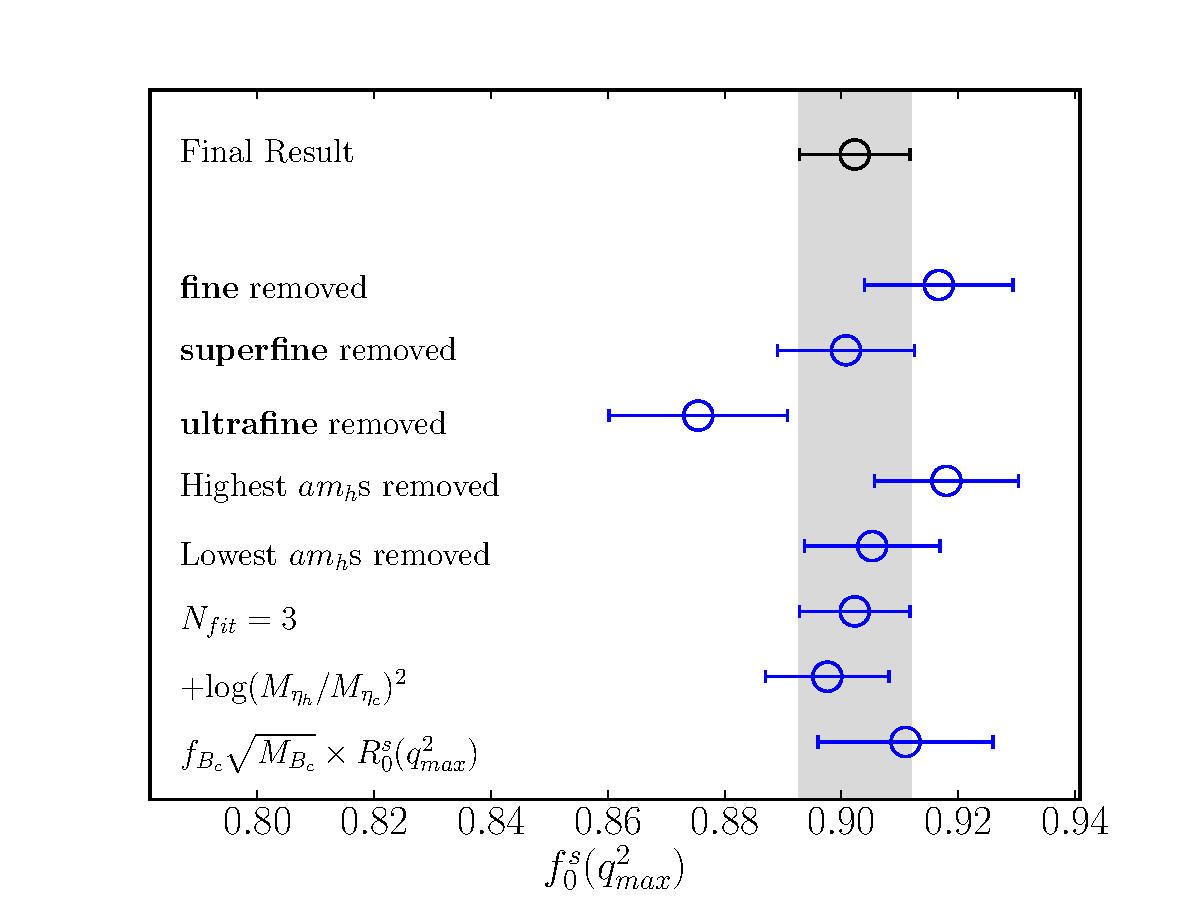
\includegraphics[width=0.85\textwidth]{images/BsDs/direct/f0q2max_stability.pdf}
  \caption{ Results of tests of the $f_0^s(q^2_{\text{max}})$ extrapolation. The top three blue points show $f_0^s(q^2_{\text{max}})$ at continuum and physical quark mass, if data from the fine, superfine or ultrafine ensembles are not used in the fit. The fourth and fifth blue points show the result if data at the highest/lowest $am_{h0}^{\text{val}}$ value on each ensemble are removed. The point labelled $N_{fit}=3$ is the result of extending the sum in \eqref{eq:mhfitfun} such that it truncates at 3 rather than 2 in each of the $i,j,k$ directions. The point labelled $+\text{log}(M_{\eta_h}/M_{\eta_c})^2$ represents the result of adding a $\rho_{2} \text{log}(M_{\eta_h}/M_{\eta_c})^2$ term in the first set of brackets in \eqref{eq:mhfitfun}, where $\rho_{2,\,n}$ are new fit parameters with the same prior distributions as $\rho_{n}$. Similarly, the point labelled $+\log(M_{\eta_c}/M_{\eta_h})/M_{\eta_h}$ gives the result of adding this term multiplied by $\rho_{2,\,n}$. The lowest point shows the result from the extrapolation of $R_0^s(q^2_{\text{max}})$, multiplied by the PDG value for $\sqrt{M_{B_c}}$ \cite{PhysRevD.98.030001} and the result of our extrapolation of $f_{B_c}$ to the physical point detailed Sec. \ref{sec:stability_BsDsstar}.
    \label{fig:directtests}}
  \end{center}
\end{figure}

\subsubsection{Non-Zero Recoil}

\begin{figure}[htb!]
  \hspace{-85pt}
  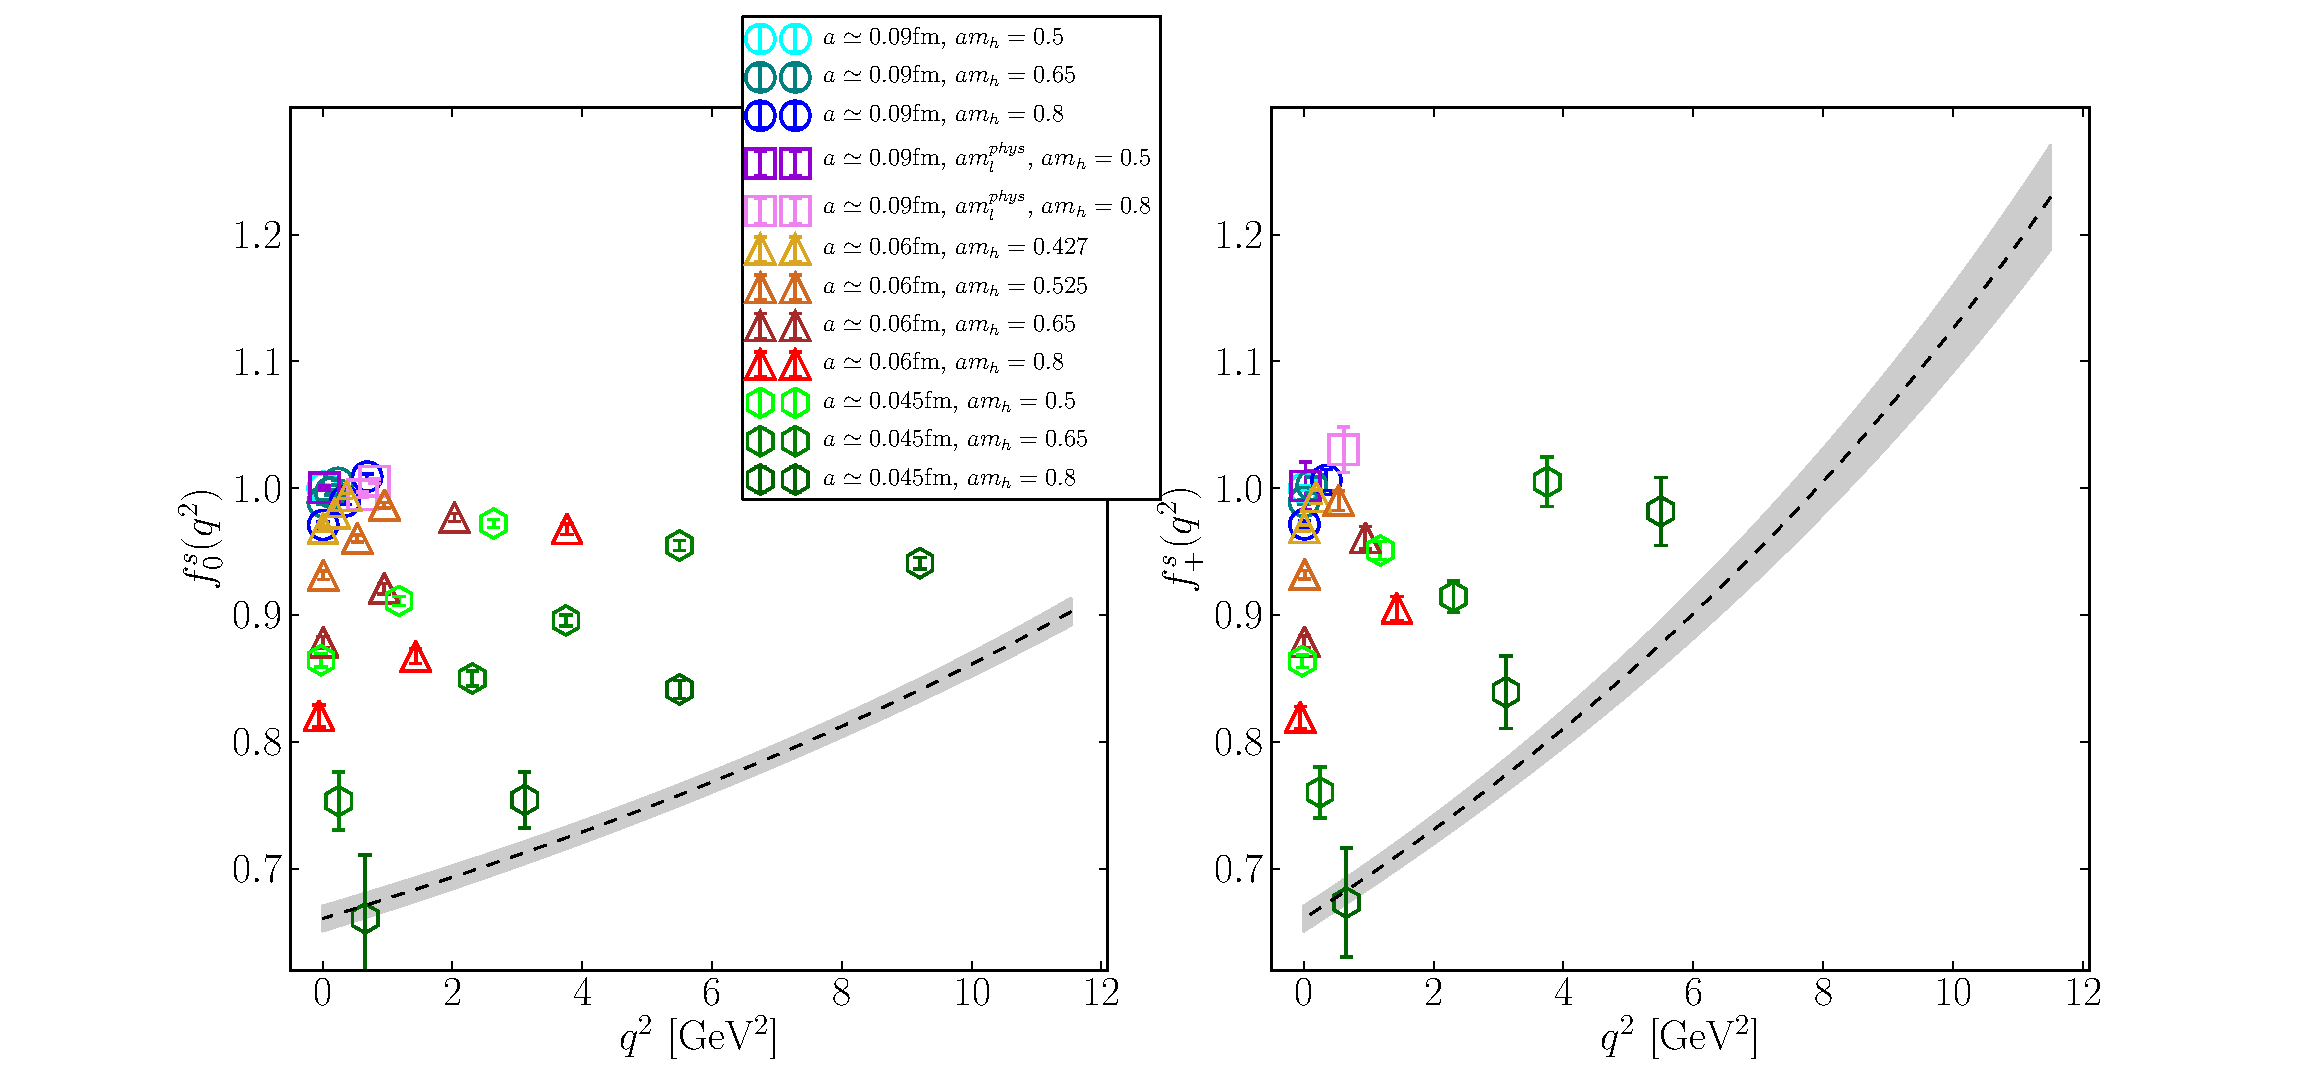
\includegraphics[width=1.40\textwidth]{images/BsDs/direct/f0fp_vsq2.pdf}
  \caption{ $f_{0,+}^s(q^2)$ against $q^2$. The grey band shows the result of the extrapolation at $a=0$ and physical quark masses. Sets listed in the legend follow the order of sets in Table \ref{tab:ensembles}. \label{fig:directdata}}
\end{figure}

\begin{figure}[htb!]
  \begin{center}
%  \hspace{-10pt}
  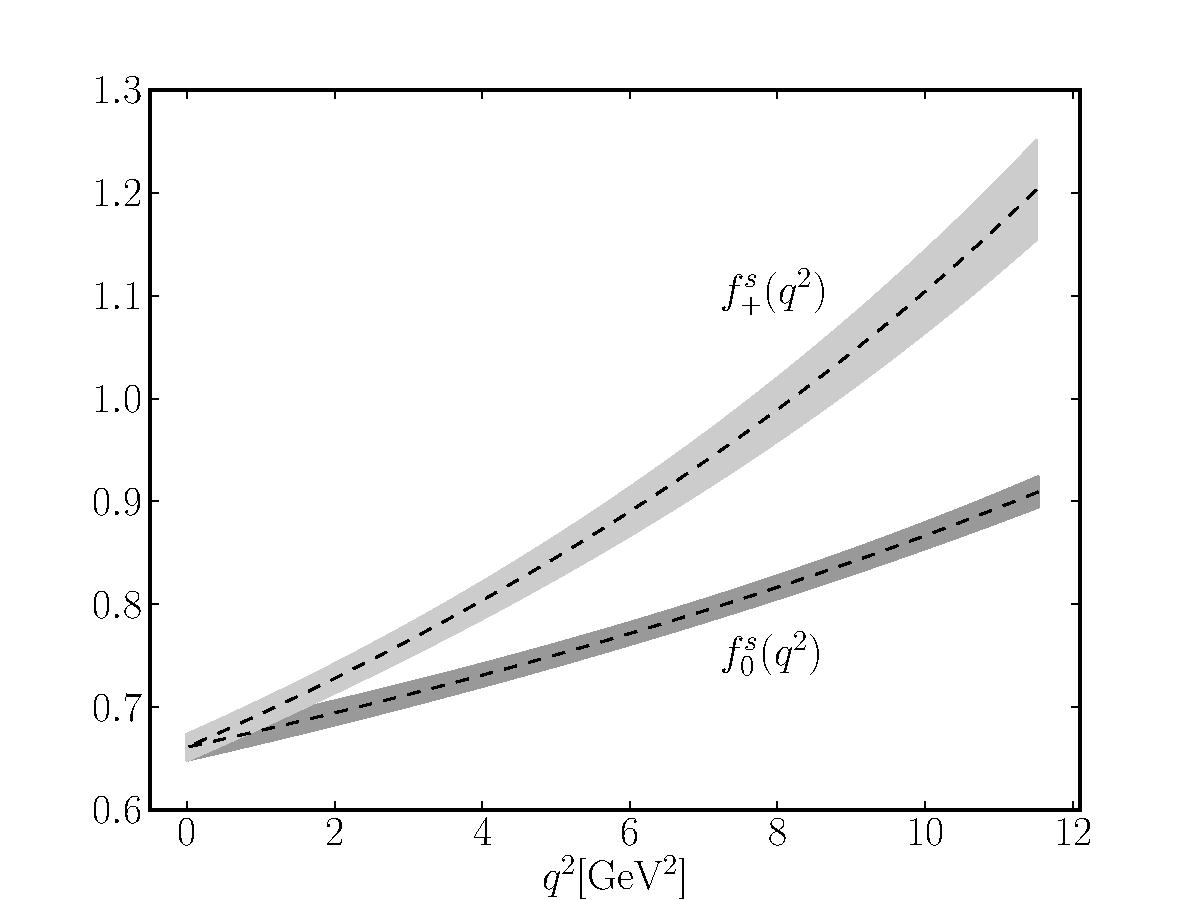
\includegraphics[width=0.85\textwidth]{images/BsDs/direct/f0fp_final.pdf}
  \caption{ Final result for $f_{0,+}^s(q^2)$ against $q^2$ at the physical point \label{fig:directfinal}.}
    \end{center}
\end{figure}

\begin{figure}[htb!]
  \hspace{-85pt}
  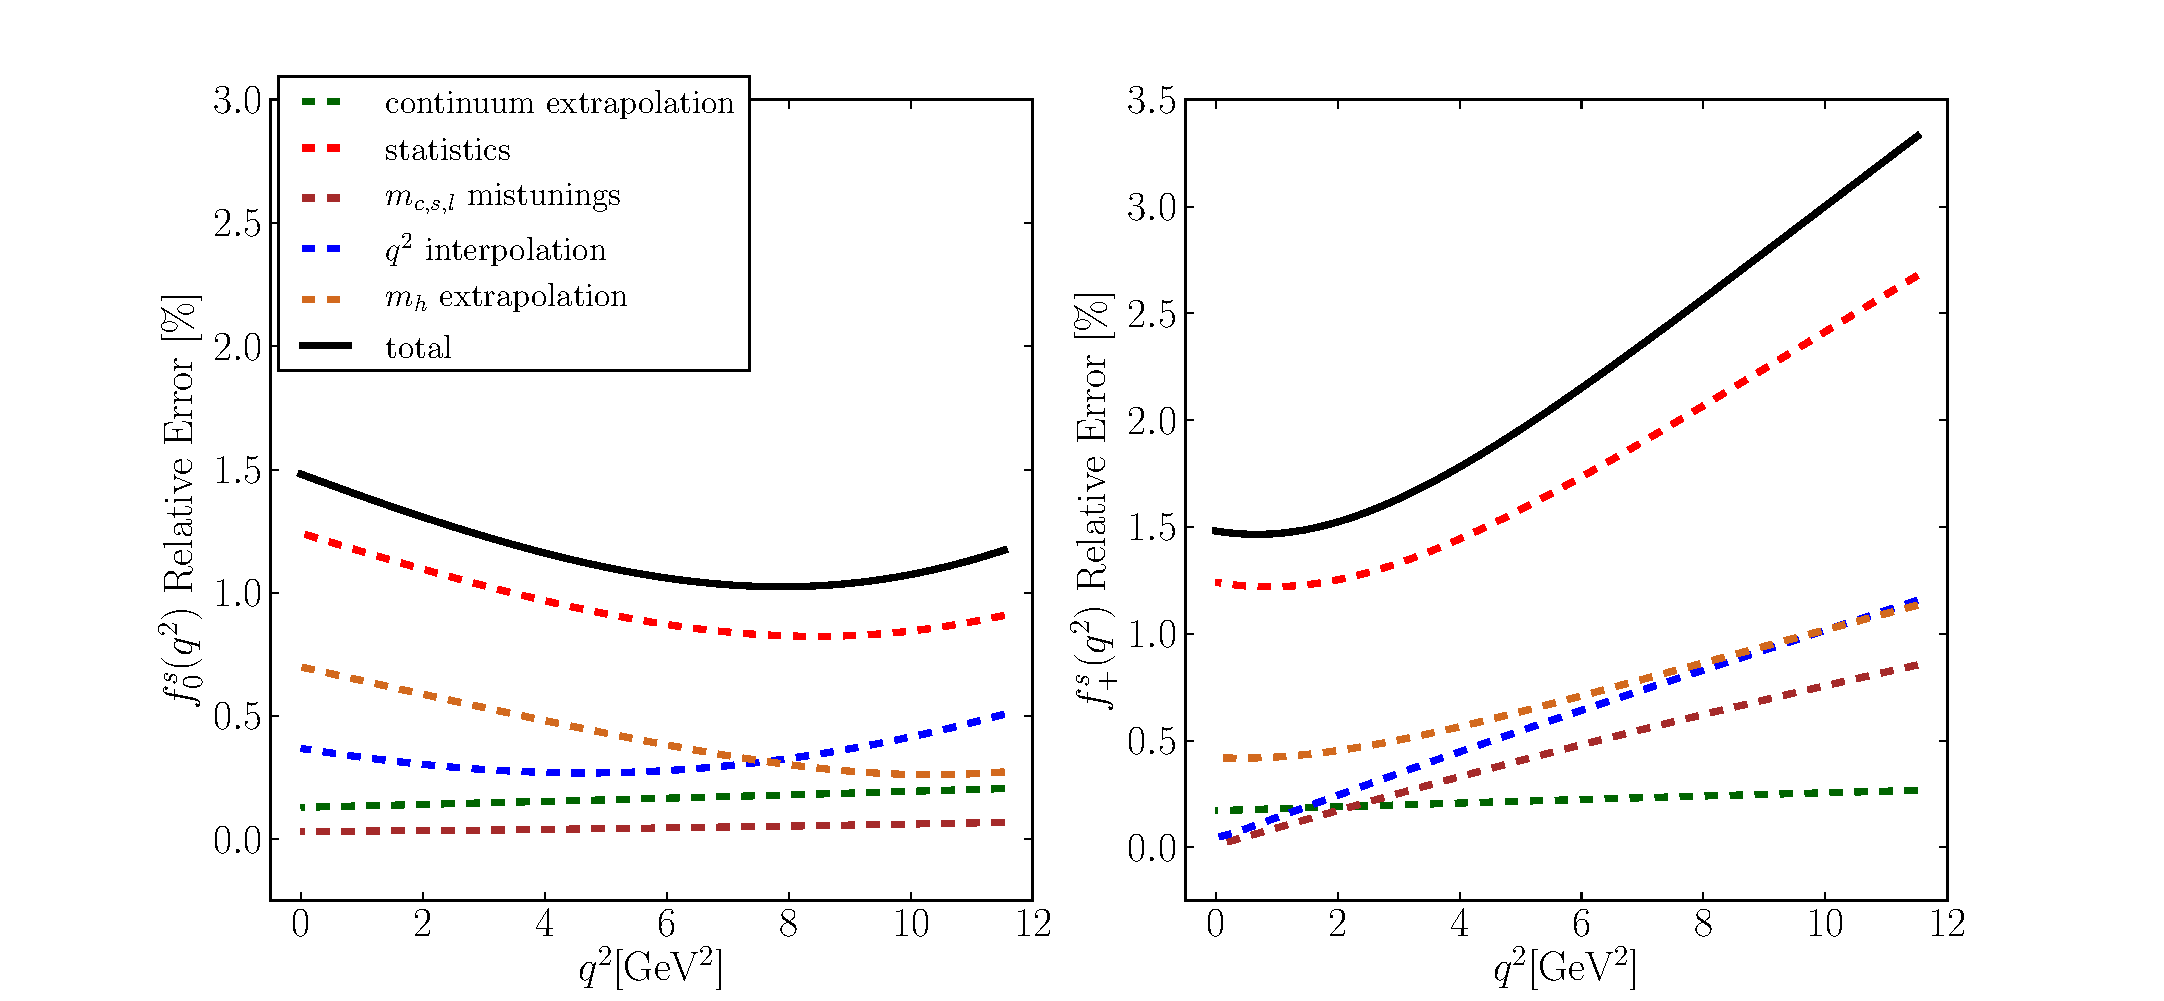
\includegraphics[width=1.4\textwidth]{images/BsDs/direct/errorbudget.pdf}
  \caption{ Error budget for $f_{0,+}^s(q^2)$ against $q^2$ \label{fig:directerrorbudget}.}
\end{figure}

Fig. \ref{fig:directdata} shows the result of the full extrapolation of the ratio throughout the $q^2$ range described in Sec. \ref{sec:extrapolation}.

Fig. \ref{fig:directfinal} shows the resulting form factors from the direct approach. In Fig. \ref{fig:directerrorbudget} we give an associated error budget for these throughout $q^2$. Statistical errors in $f^s_+$ grow in the $q^2\to q^2_{\text{max}}$ region due to the 'fine tuning' effect discussed in Sec. \ref{sec:fplus_divergence}. The effect is not as severe as in the NRQCD case since the lattice data we obtain for $f^s_+(q^2)$ is much further away from the $q^2_{\text{max}}$ point.

We take the results from the direct method as our final result, and supply the ratio method results as a consistency test, since the product of the direct method is more precise. Fig. \ref{fig:ratiovsdirect} shows the form factors resulting from the two methods on top of each other. As one can see from this plot, the results are in good agreement for all physical $q^2$ values.

\begin{figure}[htb!]
  \begin{center}
  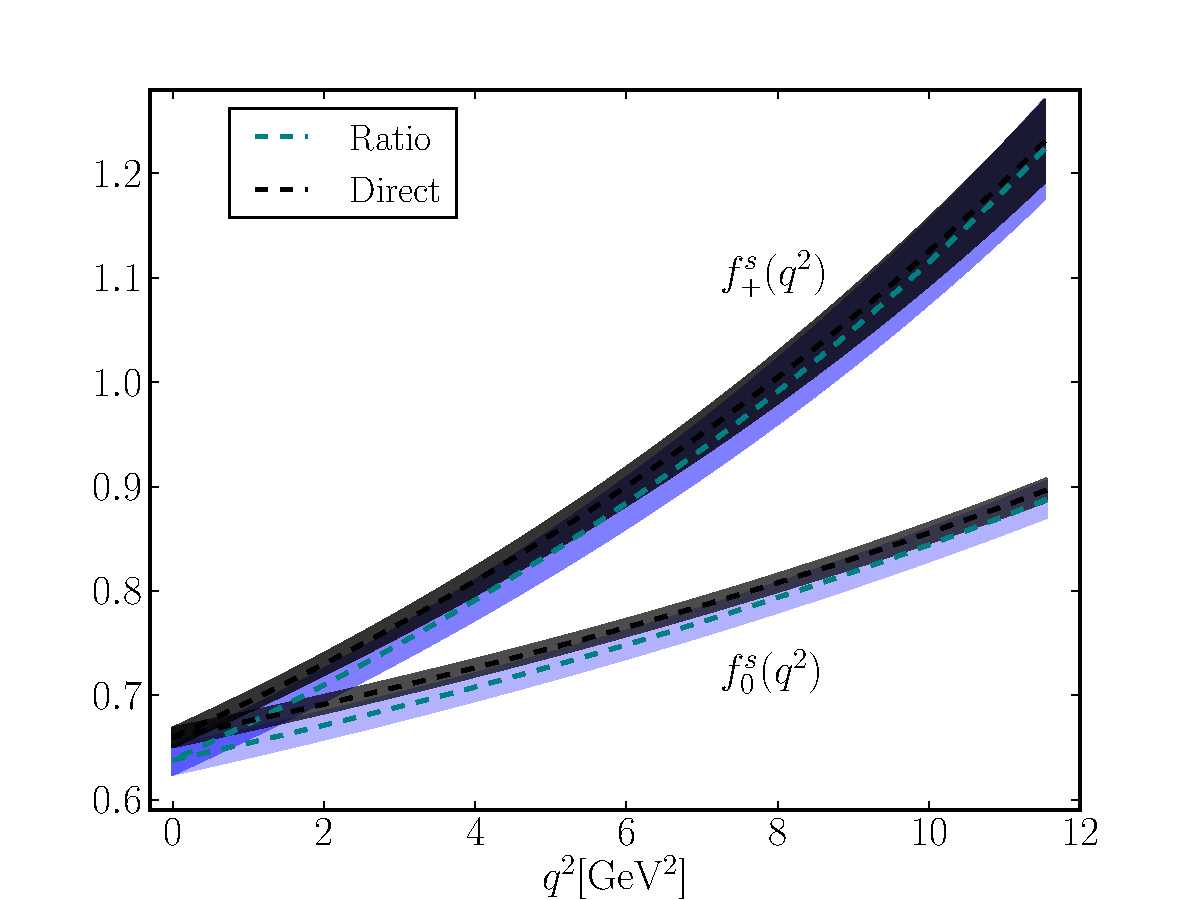
\includegraphics[width=0.85\textwidth]{images/BsDs/ratio_vs_direct.pdf}
  \caption{ Results for $f_{0,+}^s(q^2)$ against $q^2$ at the physical point, from both the ratio method and the direct method. \label{fig:ratiovsdirect}}
    \end{center}
\end{figure}

In Figure \ref{fig:nrqcd}, we show our final results (direct approach) against lattice form factors determined from the NRQCD calculation mentioned in Sec. \ref{sec:directq2max} \cite{Monahan:2017uby}. Our results are in excellent agreement with the NRQCD calculation, and are more precise for both $f^s_0(q^2)$ and $f^s_+(q^2)$ throughout all $q^2$.

\begin{figure}[htb!]
\begin{center}
  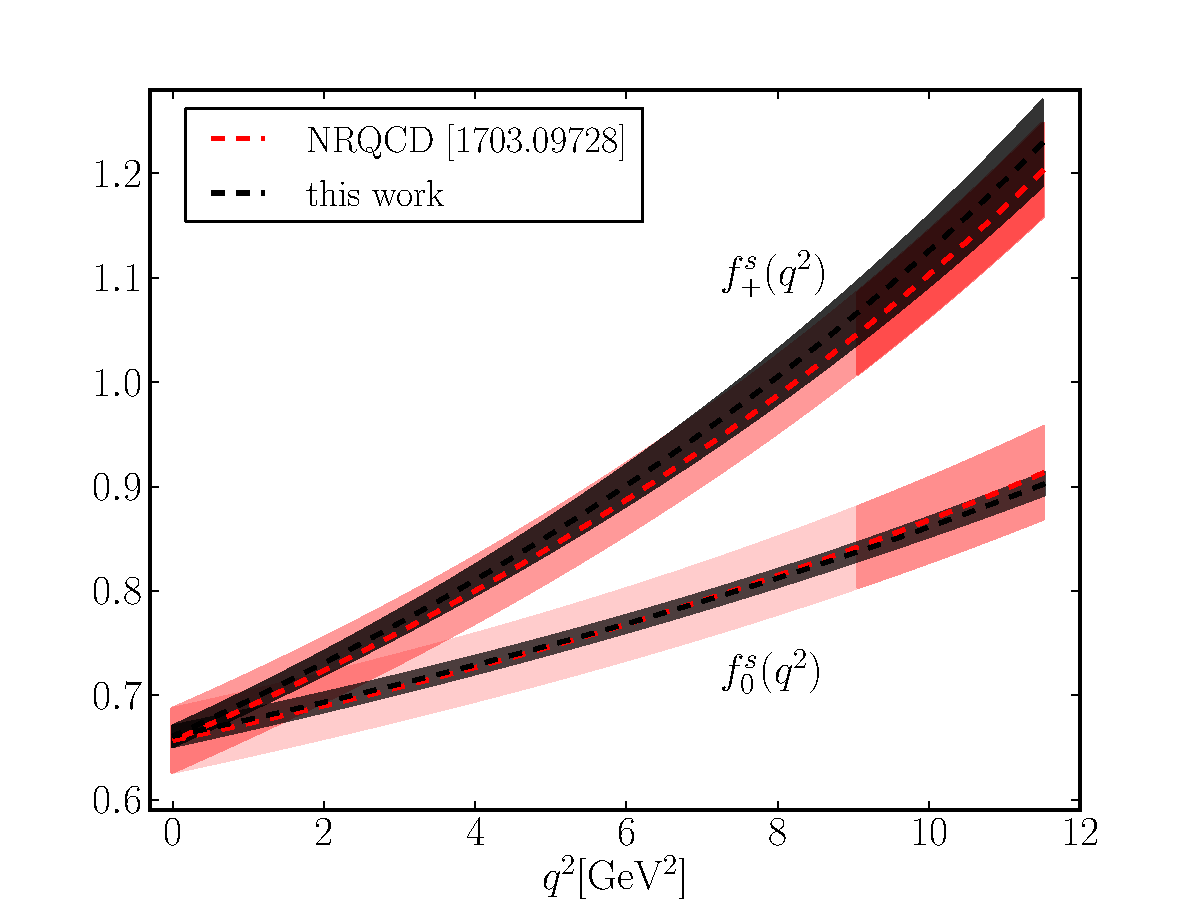
\includegraphics[width=0.85\textwidth]{images/BsDs/nrqcd_comparison.pdf}
  \caption{ Our final result for $f_{0,+}^s(q^2)$ against form factors calculated from a previous study using the NRQCD action for the $b$ quark  \cite{Monahan:2017uby}. The darker shaded region of the NRQCD band shows where lattice data was avaliable in that study, the rest of the band shows the result of an extrapolation in $q^2$ using the BCL parameterization.\label{fig:nrqcd}}
  \end{center}
\end{figure}

\FloatBarrier

\subsection{Unitarity Test}

Unitarity and crossing symmetry impose bounds on the coefficients of the BCL parameterization of $f^s_{0,+}(q^2)$, $\{a_n\}$ \cite{PhysRevD.4.725,PhysRevD.3.2807}. As another consistency test, we show here that the coefficients found in our fit satisfy these bounds.

To obtain bounds on the BCL coefficients, one must relate them to those of a different parameterization, that of Boyd, Grinstein and Lebed (BGL) \cite{GLENNBOYD1996493}:
\begin{align}
  f^s(q^2) = {1\over B(z)\phi(z)} \sum^N_{n\geq 0} b_n z^n.
\end{align}
$B(z)$ is known as the Blashke factor:
\begin{align}
  B(z) = { z - z_* \over 1 - z z_* }\,,
\end{align}
where $z_* = z(M^2_{B_c^0})$ for $f_0^s$, or $z(M^2_{B_c^*})$ for $f_+^s$. $\phi(z)$ is the outer function:
\begin{align}
  \phi(z) &= M_{B_s}^{2-s} 2^{2+p} \sqrt{\kappa n_f}
  \left[ {M_{D_s}\over M_{B_s}} (1+z)\right]^{s-3/2} \nonumber \\
  \times &\left[ (1-z)\left(1+{M_{D_s}\over M_{B_s}}\right)+2\sqrt{M_{D_s}\over M_{B_s}}(1+z)\right]^{-s-p}\,.
\end{align}
In the $f^s_0$ case, $\kappa=12\pi M^2_{B_s}\chi_A$, $p=1$,\,$s=3$. In the $f^s_+$ case, $\kappa=6\pi M^2_{B_s} \chi_V$, $p=3$,\,$s=2$. The quantities $\chi_{V,A}$ are the once-subtracted dispersion relations at $q^2=0$ for vector and axial $b\to c$ currents respectively, computed in \cite{GLENNBOYD1996493} to be $\chi_V = 5.7\times 10^{-3}/m_b^2$ and $\chi_A = 9.6\times 10^{-3}/m_b^2$.

The BGL coefficients, $\{ b_n \}$, obey the unitarity constaint
\begin{align}
  \sum_{m=0}^{\infty} |b_m|^2 \leq 1
  \label{eq:unitarity1}
\end{align}
by construction of the parameterization. To see how this applies to the BCL coefficients $\{ a_n \}$, one must relate them to $\{ b_m \}$ by equating the two parameterizations to find
\begin{align}
  \label{eq:BCL-BGL}
  \sum^M_{m=0} b_m z^m = \psi(z) \sum_{n=0}^N a_n z^n,
\end{align}
where $\psi(z)$ is given by
\begin{align}
  \psi(z) = { M_{\text{pole}}^2 \over 4(t_+ - t_0) } \phi(z) {(1-z)^2(1-z_*)^2\over (1-zz_*)^2 },
\end{align}
where $M_{\text{pole}}=M_{B_c^0}$ in the $f^s_0$ case and $M_{B_c^*}$ in the $f^s_+$ case. Expanding $\psi(z)$ around $z=0$, comparing coefficients of $z$ in \eqref{eq:BCL-BGL}, and imposing the constraint \eqref{eq:unitarity1}, we arrive at a constraint for the BCL coefficients
\begin{align}
    \label{eq:unitarity2}
    &\mathcal{B} \equiv \sum_{j,k=0}^{L,L} B_{jk} a_j a_k \leq 1\,, \\
    &B_{jk} = \sum_{n=0}^{\infty} \eta_n \eta_{n+|j-k|}\,.
        \label{eq:Bmatrix}
\end{align}
where $\{\eta_n\}$ are the taylor coefficients of $\psi(z)$.

$\psi(z)$ is bounded on the closed disk $|z|<1$, so its Taylor coefficients are rapidly decreasing. We computed values for $B_{jk}$ by truncating the sum in its definition \eqref{eq:Bmatrix} at 100. These values are given in Table \ref{tab:Bmatrix}. With these $B_{jk}$ values, and the $a_n$ coefficients at the physical point from our fit (via the direct method), we find
\begin{align}
  \nonumber
  \mathcal{B}_0 = 0.0008(15)\,,
  \\ \mathcal{B}_+ = 0.0204(66)\,.
  \nonumber
\end{align}
These comfortably satisfy the unitarity bound. Additionally, as discussed in \cite{BECHER200661}, the leading contributions to $\mathcal{B}_{0,+}$ are of order $(\Lambda_{\text{QCD}}/m_b)^3 \simeq 10^{-3}$ in HQET. This expectation is approximately fulfilled by our result.

\begin{table}[htb!]
  \begin{center}
    \begin{tabular}{c c c c}
      \hline
      & $B_{00}$ & $B_{01}$ & $B_{02}$ \\ [0.5ex]
      \hline
      $f^s_0$ & 0.00186 & -0.000258 & -0.000703 \\ [0.5ex]
      $f^s_+$ & 0.00179 & -0.000367 & 0.00108 \\ [0.5ex]
      \hline
    \end{tabular}
  \end{center}
  \caption{Numerical values for $B_{jk}$ appearing in the unitarity bound for BCL coefficients, defined in \eqref{eq:Bmatrix}, for the $f^s_0$ and $f^s_+$ cases. The rest of the elements can be obtained from these using the properties $B_{j(j+k)}=B_{0k}$ and $B_{jk}=B_{kj}$. \label{tab:Bmatrix}}
\end{table}


\subsection{$R_{D_s}$}

%% \begin{figure}[htb!]
%%   \begin{center}
%%   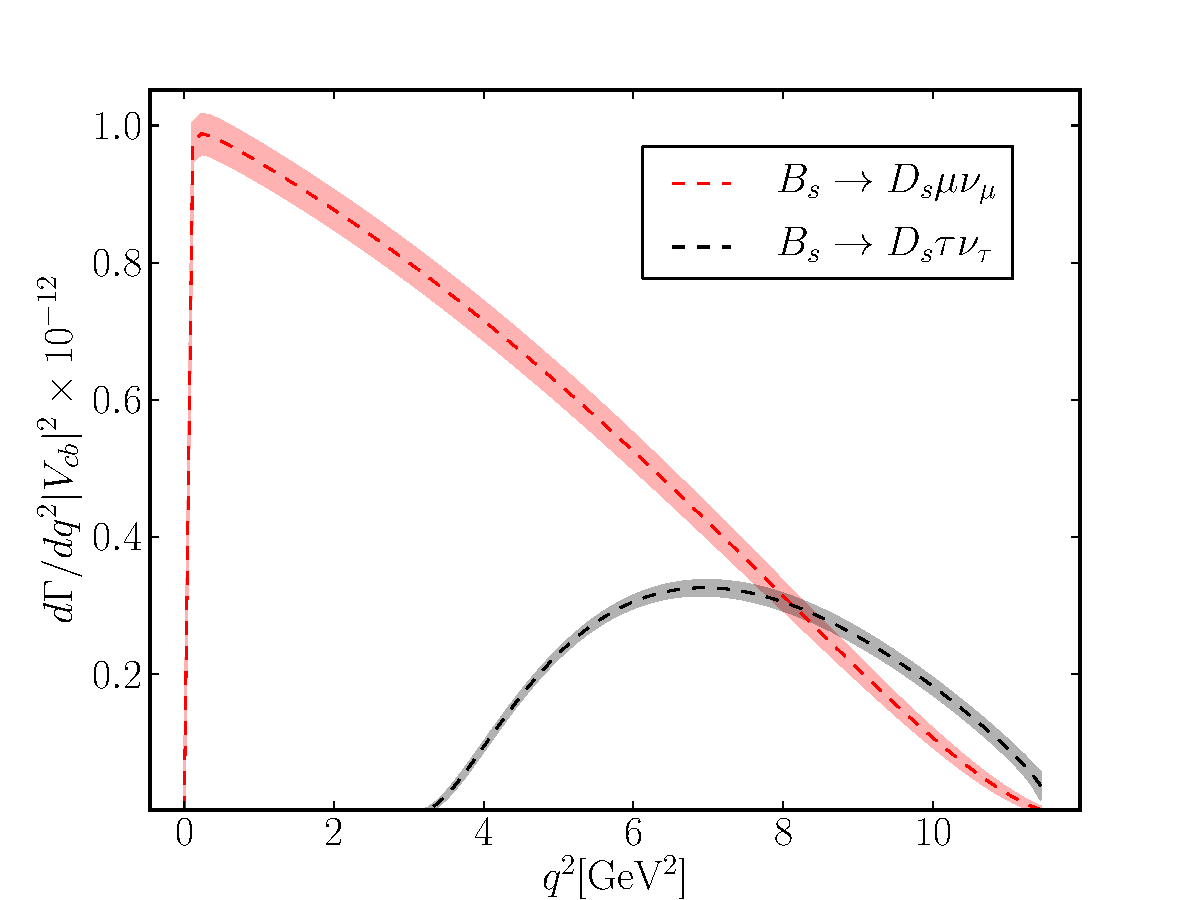
\includegraphics[width=0.75\textwidth]{images/BsDs/direct/branchingfraction.pdf}
%%   \caption{Decay rates for the $B_s\to D_s\mu\nu_{\mu}$ and $B_s\to D_s\tau\nu_{\tau}$ decays, derived using form factors calculated in this work.}
%%   \end{center}
%% \end{figure}

Using our calculated form factors $f^s_{0,+}(q^2)$, we can produce a new prediction for the quantity
\begin{align}
  R_{D_s} = {\mathcal{B}(B_s\to D_s \tau \nu_{\tau})\over
    \mathcal{B}(B_s\to D_s l \nu_{l})}\,,
\end{align}
where $l=e$ or $\mu$ (the ambiguety between $e$ and $\mu$ is negligable in comparison to the current precision on $R_{D_s}$). As mentioned in the introduction, the analagous quantities $R_{D}$ and $R_{D^*}$ are in tension between SM prediction and experimental measurement. There is, at time of writing, no published measurement of $R_{D_s}$, providing an opportunity for lattice QCD to give a clear prediction of the value of $R_{D_s}$ expected by the SM.

Armed with form factors from a lattice QCD calculation, one can immediately produce an $R_{D_s}$ determination by taking the ratio of SM branching fractions \eqref{eq:branchingfraction} between the $l=\tau$ and $l=\mu,e$ cases. $|V_{cb}|$ and $\eta_{EW}$ cancel in the ratio.

A lattice prediction has already been made in \cite{Monahan:2017uby} of $R_{D_s}|_{\text{SM}} = 0.301(6)$. We here report a new prediction:
\begin{align}
  R_{D_s}|_{\text{SM}} = 0.2985(51).
  \label{eq:RDs}
\end{align}
To arrive at this prediction we averaged over the $l=e$ and $l=\mu$ cases. We give an error budget for this result in terms of errors from our lattice calculation in table \ref{RDs_budget}. As a check we also compute $R_{D_s}$ using form factors from resulting from the ratio method tofind $R_{D_s}|_{\text{SM}} = 0.2999(58)$.

\begin{table}[htb!]
  \begin{center}
    \begin{tabular}{c c}
      \hline
      Source & \% Fractional Error \\ [0.5ex]
      \hline
      Statistics & 1.27  \\ [1ex]
      Scale Setting & 0.41  \\ [1ex]
      Kinematic Interpolation & 0.85  \\ [1ex]
      $m_h \to m_b$, & 0.74  \\ [1ex]
      $a\to 0$ & 0.06  \\ [1ex]
      Quark Mass Mistuning & 0.02 \\ [1ex]
      \hline
      Total & 1.70 \\ [1ex]
      \hline
    \end{tabular}
  \end{center}
  \caption{Error budget for $R_{D_s}|_{\text{SM}}$.\label{RDs_budget}}
\end{table}

%% \section{$h^s_+(1)$ and HQET low energy constants}

%% Recall from Sec. \ref{sec:Luke} that there is an alternative parameterization of pseudoscalar-to-pseudoscalar transition amplitudes, given in Eq. \eqref{eq:pseudoscalar_hqet}, motivated by HQET. The form factor $h^s_+$ is protected by Luke's theorem at zero recoil and can be written as
%% \begin{align}
%%   \label{eq:h+}
%%   &h^s_+(1) = \eta_V \left[ 1 - l^s_P \left( {1\over 2m_h} - {1\over 2m_c} \right)^2 \right] + \mathcal{O}\left( \, {1\over m_c^n m_h^m}, \, n+m\geq 3 \, \right).
%% \end{align}
%% This invites an extrapolation of $h^s_+(1)$ through $m_h$ in the same way as $h_{A_1}^s(1)$ was extrapolated. We perform this for two reasons - to find a new estimation of $l_P^s$, and to supply another consistency test for the $m_h$ extrapolation of $f_0(q^2_{\text{max}})$.

%% We perform the $h_+(1)$ extrapolation using the fit form
%% \begin{align}
%%   \label{eq:h+_fitform}
%%   h^s_+(1)|_{\text{fit}} =&\, \eta_V \left[ 1 - l^s_P \left( {1\over M_{\eta_h}} - {1\over M_{\eta_c}} \right)^2 \right]
%%   + \mathcal{N}_{\text{disc}} + \mathcal{N}_{\text{mistuning}}.
%% \end{align}
%% where $\mathcal{N}_{\text{disc}}$ is defined in \eqref{eq:fitfun_hA1}, and $\mathcal{N}_{\text{mistuning}}$ in \eqref{eq:mistuning_BsDsstar}. Experience from the extrapolation of $h_{A_1}^s(1)$ shows us that $M_{\eta_h}/2$ is a suitable proxy for the heavy quark mass at current precision of the lattice data. $\eta_V$ has a 1-loop expression \cite{PASCHALIS1983473}:
%% \begin{align}
%%   \eta_V(m_h) = 1 - {3 \alpha_s(m_b) \over 4\pi} \left( {m_h+m_c\over m_h-m_c} \log\left({m_c\over m_h}\right) - {3\over 2} \right),
%% \end{align}
%% and has been computed to 2-loop to have the value $\eta_V = 1.022(4)$ \cite{PhysRevLett.76.4124}. Similarly to $\eta_A$, this varies weakly with $m_h$, the variance of this through the $m_c \leq m_h \leq m_b$ range is illustrated in Fig. \ref{fig:etaAV}. Like in the $h^s_{A_1}(1)$ case, we attempted the fit with an extra $(1+\rho \log(M_{\eta_c}/M_{\eta_h}))$ factor multiplying $\eta_V$ ($\rho$ is a fit parameter with prior distribution $0\pm 1$), and this reduced the Bayes factor by a factor of 16. So the $\eta_V$ dependence on $m_h$ can be safely ignored.

%% We did, however, find that there is not enough freedom in a fit to the above form to achieve $\chi^2/N_{\text{dof}} \leq 1$. The only way to obtain a good fit is to promote $\eta_V$ to a fit parameter, with prior distribution $1\pm \alpha_s^2$, where we take $\alpha_s=0.22$. All other priors are given the same distributions as in the $h^s_{A_1}(1)$ case, except for $d_{ijk}$ which are each given the prior $0\pm 1$.

%% \begin{figure}[htb!]
%%   \begin{center}
%%     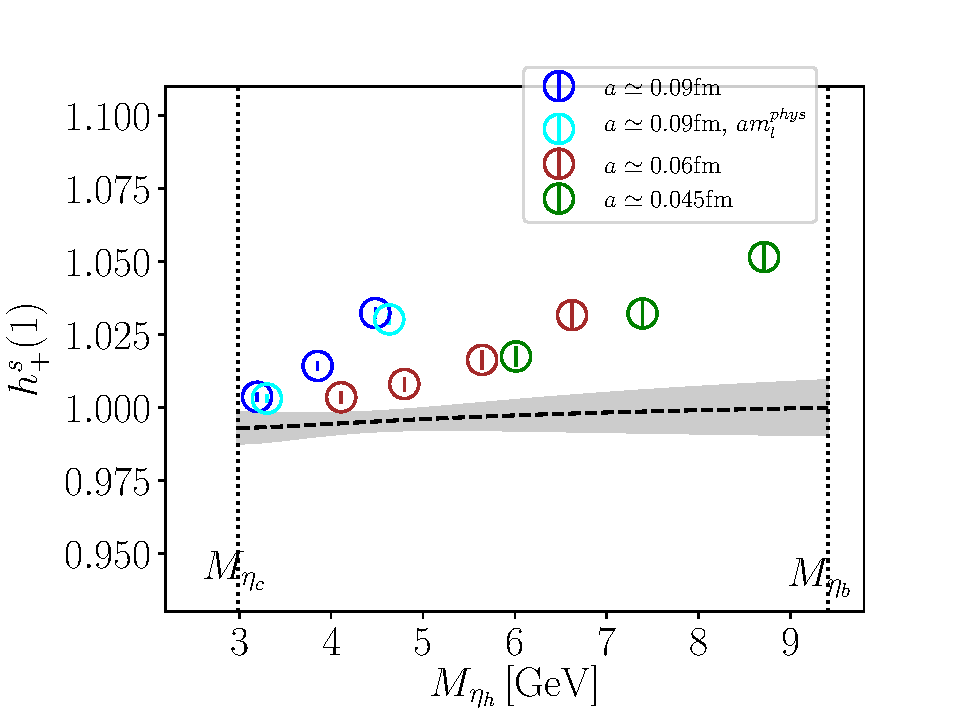
\includegraphics[width=0.85\textwidth]{images/BsDs/hplus_vsmh.pdf}
%%     \caption{Extrapolation of $h^s_+(1)$ through $M_{\eta_h}$. The grey band shows the $a\to 0$ and physical charm, strange and light quarks result. \label{fig:hplus_extrap}}
%%   \end{center}
%% \end{figure}

%% The extrapolation is illustrated in Fig. \ref{fig:hplus_extrap}. The result for $h^s_+(1)$ at continuum and all physical quark masses is
%% \begin{align}
%%   h_+^s(1) = 0.9998(81)_{\text{stat}}(45)_{\text{sys}}.
%% \end{align}
%% The fit finds new non-perturbative values for
%% \begin{align}
%%   \eta_V = 0.9931(52) \quad,\quad l_P^s = -0.07(13) \text{GeV}^2.
%% \end{align}
%% Our estimate for $l_P^s$ here is consisistent with the $l_P^s$ value found from the $h^s_{A_1}(1)$ study of $l_P^s=-0.25(20)$GeV$^2$ (in the sense that neither of them say anything really).

%% From this $h^s_+$ result at the physical point we can produce a new $f^s_0(q^2_{\text{max}})$ value for comparison with our final result:
%% \begin{align}
%%   f^s_0(q^2_{\text{max}})|_{h_+} = {2\sqrt{ M_{B_s}M_{D_s} }\over M_{B_s}+M_{D_s}} h^s_+(1) = 0.8860(82).
%% \end{align}
%% This is in a mild $1.7\sigma$ tension with our result from the direct $f^s_0(q^2_{\text{max}})$ extrapolation given in Eq. \eqref{eq:f0s_direct}.

\section{Conclusions}
\label{sec:BsDs_conclusions}

We have produced a fully non-perturbative lattice QCD prediction of the scalar and vector form factors for the $B_s\to D_s l\nu$ decay throughout the entire $q^2$ range (Fig. \ref{fig:directfinal}, see Sec. \ref{sec:reconstructing_formfactors} to reconstruct), and a value for $R_{D_s}$ (Eq. \eqref{eq:RDs}). Our results are statistics dominated. In this calculation we used correlation functions from 3 lattice spacings, including an ensemble with an approximately physical light quark mass, and learned the $b$-mass dependence of the form factors by obtaining data at 12 different heavy quark masses.

Our results supply an independent check on the NRQCD formalism for computing pseudoscalar$\to$pseudoscalar form factors. Our results validate the $q^2$-extrapolation from high $q^2$ lattice data used in the NRQCD case since our formalism produced lattice data throughout all $q^2$. We have also shown that the systematic error assigned to the NRQCD results to account for perturbative matching and truncation of the $1/m$ series in the NRQCD-HISQ current is sufficient. Our results are however more precise and do not rely on the assumptions implicit in the NRQCD formalism.

Our calculation has shown that a heavy-HISQ determination of the $B\to Dl\nu$ form factors is very plausible. Such a calculation could use an essentially identical process as given here, with the strange valence quark simply replaced with a light one. Perhaps correlation functions from additional ensembles with smaller light quark masses would be necessary to resolve the dependence of the form factors on the light mass. Also, more statistics would likely be necessary, since the presence of a light valence quark increases the noise in the lattice data, and statistics is already the dominant uncertainty in this calculation.

\FloatBarrier

\section{Reconstructing Form Factors}
\label{sec:reconstructing_formfactors}

This section gives the necessary information to reproduce the functional form of the form factors through $q^2$ reproduced in this work. We here express the form factors in terms of the BCL parameterization \cite{Bourrely:2008za}:
\begin{align}
  \label{eq:BCLappendix}
  &f^s_0(q^2) = {1\over 1 - {q^2\over M_{B_c^0}^2} } \sum_{n=0}^{2} a_n^0 z^n(q^2), \\
  \nonumber
  &f^s_+(q^2) = {1\over 1 - {q^2\over M_{B_c^*}^2} } \sum_{n=0}^{2} a_n^+ \left( z^n(q^2) - {n\over 3} (-1)^{n-3} z^3(q^2) \right), \nonumber
\end{align}
where the function $z(q^2)$ is defined by defined by
\begin{align}
  z(q^2) = {\sqrt{t_+ - q^2} - \sqrt{t_+} \over \sqrt{t_+ - q^2} + \sqrt{t_+} }\,,
\end{align}
and $t_+ = (M_{B_s}+M_{D_s})^2$ (one should take the PDG 2018 values for these masses). For the position of the poles, one can use $M_{B_c^0} = 6.70390(80)$GeV and $M_{B_c^*} = 6.28030(80)$GeV. The coefficients $a_n^{0,+}$ found from our fit, along with their covariance, is given in table \ref{tab:coeffs}.

\begin{table}[htb!]
\begin{center}
\begin{tabular}{ c c c c c c c }
\hline
 & $a^0_0$ & $a^0_1$ & $a^0_2$ & $a^+_0$ & $a^+_1$ & $a^+_2$\\ [0.5ex]
\hline
 & 0.66097 & -0.26421 & -0.26158 & 0.66097 & -3.17196 & 0.10935\\ [1ex]
\hline
 & 0.00016 & 0.00217 & 0.00125 & 0.00016 & 0.00014 & 0.00001\\ [1ex]
 &  & 0.06838 & 0.18373 & 0.00217 & 0.01578 & -0.00031\\ [1ex]
 &  &  & 3.47982 & 0.00125 & 0.18432 & -0.00606\\ [1ex]
 &  &  &  & 0.00016 & 0.00014 & 0.00001\\ [1ex]
 &  &  &  &  & 0.27937 & 0.09825\\ [1ex]
 &  &  &  &  &  & 4.06414\\ [1ex]
\hline
\end{tabular}
    \caption{Our results for $z$-coefficients in the BCL parameterization \eqref{eq:BCLappendix}. The first row gives mean values, and the rest of the table gives the covarance matrix associated with these parameters. \label{tab:coeffs}}
\end{center}
\end{table}




%% \section{$f_{B_c}$ Determination}
%% \label{sec:fHc}

%% In our ratio method described in sec. \ref{sec:ratiomethod}, we need a determination of $f_{B_c}$ to multiply into $R_{0,+}^s(q^2)$ in order to isolate the form factors. Here we detail our determination of $f_{B_c}$.

%% We obtain values for $f_{H_c}$ on each ensemble and with each heavy mass given in tables \ref{tab:ensembles} and \ref{tab:simulation}.
%% \begin{align}
%%   \label{eq:fitfun_ratio}
%%   \nonumber
%%   f_{H_c}|_{\text{fit}} = &\left({\alpha_s(M_{\eta_h})\over\alpha_s(M_{\eta_c})}\right)^p M_{\eta_h}^{-1/2} \times \\ &\sum_{i,j,k=0}^{2,2,2} d_{ijk} \left({\Lambda_{\text{QCD}}\over M_{\eta_h} }\right)^{i} \left({ am^{\text{val}}_{h0} \over \pi }\right)^{2j} \left({ am^{\text{val}}_{c0} \over \pi }\right)^{2k} \\
%%   &+ \mathcal{N}_{\text{mistuning}}.
%%   \nonumber
%% \end{align}
%% $\alpha_s(M)$ is the QCD coupling constant evaluated at scale $M$. $p$ is a fit parameter with prior distribution $-2/9\pm 1/9$. The $M_{\eta_h}^{n/2}$ accounts for the leading order dependance of $f_{H_c}$ in HQET, and the $\alpha_s$ ratio comes from matching between QCD and HQET of $f_{H_c}$. $\mathcal{N}_{\text{mistuning}}$ is defined in \ref{eq:mistuning}.

%% The extrapolation in $f_{H_c}$ is shown in fig. \ref{fig:fHc_vsmh}. We here include the result from a previous heavy-HISQ determination of $f_{B_c}$ on 2+1 gauge ensembles \cite{McNeile:2012qf}. Our result is slightly higher than theirs, since their study used only unphysically heavy light quarks ($m_l/m_s\simeq=0.2$), and did not control for associated effects.

%% \begin{figure}[htb!]
%%   \hspace{-20pt}
%%   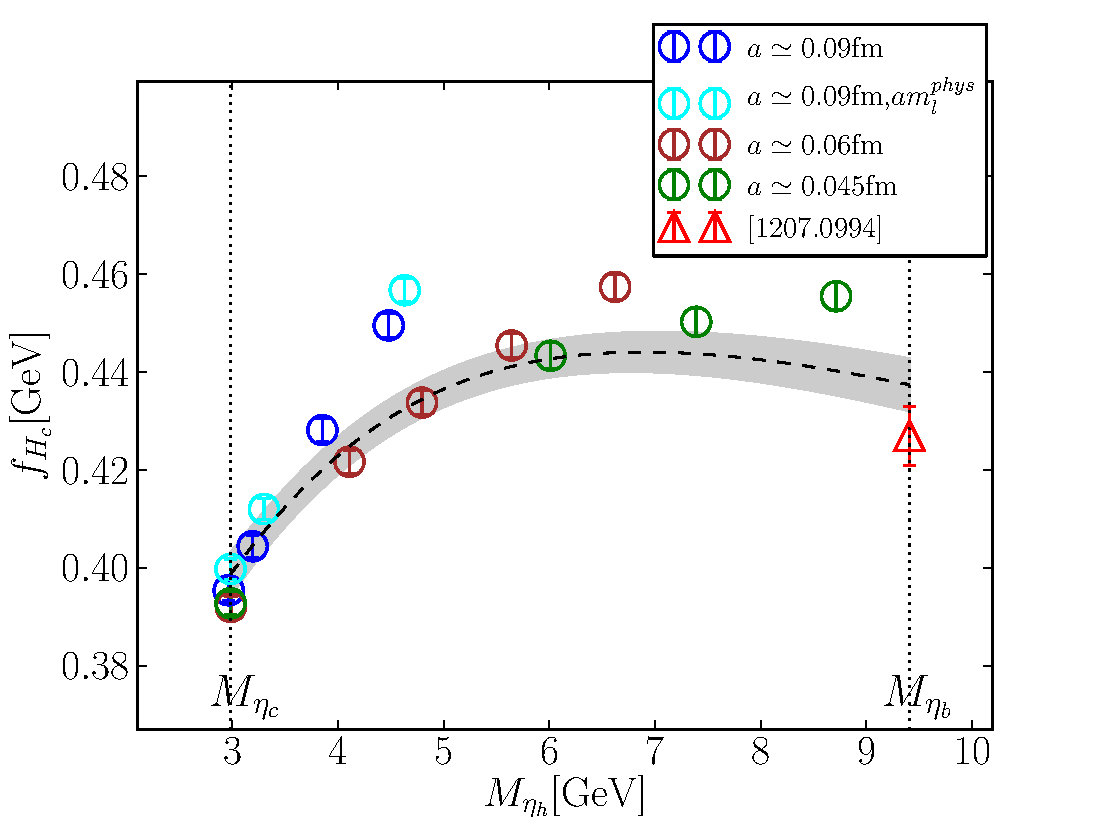
\includegraphics[width=0.53\textwidth]{images/BsDs/ratio/fHc_vsmh.pdf}
%%   \caption{ $f_{H_c}$ against $M_{\eta_h}$ (a proxy for the heavy quark mass). The grey band shows the result of the extrapolation at $a=0$ and physical $l$,$s$ and $c$ masses. Sets listed in the legend follow the order of sets in table \ref{tab:ensembles}. The red point shows the result from a previous heavy-HISQ determination of $f_{B_c}$ on 2+1 gauge ensembles \cite{McNeile:2012qf}\label{fig:fHc_vsmh}}.
%% \end{figure}

\section{Numerical Values for Lattice Results}
\label{sec:tables}

In this section we give two tables, consisting of all numerical results for form factors, ratios $R_{0,+}^s(q^2)$, masses, energies and decay constants required for the extrapolations performed to the physical point. Table \ref{tab:masses} gives results results relevant to all $q^2$ values, while \ref{tab:kinetic} gives results that vary over $q^2$.

%% \begin{table*}[htb!]
%%   \begin{center}
%%     \begin{tabular}{ c c c c c c c c c }
%%       \hline
%%       Set & $am_h^{\text{val}}$ & $M_{H_s}$& $M_{D_s}$& $M_{H_c}$& $f_{H_c}$& $M_{\eta_h}$& $M_{\eta_c}$& $M_{\eta_s}$\\ [0.5ex]
%%       \hline
%%       0 & 0.5 & 2.084(12) & 1.959(11) & 3.082(17) & 0.4045(23) & 3.195(18) & 2.968(17) & 0.6815(38)\\ [0.5ex]
%%       & 0.65 & 2.443(14) &  & 3.416(19) & 0.4282(24) & 3.854(22) &  & \\ [0.5ex]
%%       & 0.8 & 2.782(16) &  & 3.737(21) & 0.4496(25) & 4.481(25) &  & \\ [0.5ex]
%%       \hline
%%       1 & 0.5 & 2.143(11) & 1.970(10) & 3.144(17) & 0.4121(22) & 3.301(17) & 2.985(16) & 0.6846(36)\\ [0.5ex]
%%       & 0.8 & 2.865(15) &  & 3.823(20) & 0.4567(24) & 4.633(24) &  & \\ [0.5ex]
%%       \hline
%%       2 & 0.427 & 2.580(15) & 1.971(11) & 3.556(20) & 0.4217(24) & 4.110(23) & 2.988(17) & 0.6900(39)\\ [0.5ex]
%%       & 0.525 & 2.947(17) &  & 3.907(22) & 0.4338(25) & 4.797(27) &  & \\ [0.5ex]
%%       & 0.65 & 3.396(19) &  & 4.342(24) & 0.4455(25) & 5.644(32) &  & \\ [0.5ex]
%%       & 0.8 & 3.911(22) &  & 4.846(27) & 0.4574(26) & 6.623(37) &  & \\ [0.5ex]
%%       \hline
%%       3 & 0.5 & 3.593(22) & 1.970(12) & 4.530(28) & 0.4434(27) & 6.013(37) & 2.986(18) & 0.6889(42) \\ [0.5ex]
%%       & 0.65 & 4.315(26) &  & 5.238(32) & 0.4503(28) & 7.390(45) &  & \\ [0.5ex]
%%       & 0.8 & 5.004(31) &  & 5.919(36) & 0.4555(28) & 8.713(53) &  & \\ [0.5ex]
%%       \hline
%%     \end{tabular}
%%     \caption{}
%%   \end{center}
%% \end{table*}

\begin{sidewaystable}
  \begin{center}
    \begin{tabular}{ c c c c c c c c c }
      \hline 
      Set & $am_{h0}^{\text{val}}$ & $aM_{H_s}$ & $aM_{D_s}$ &  $aM_{H_c}$ & $af_{H_c}$ & $aM_{\eta_h}$ & $aM_{\eta_c}$ & $aM_{\eta_s}$ \\ [0.5ex]
      \hline 
      0 &0.5 &0.95976(11) &0.90222(10) &1.419515(41) &0.186299(70) &1.471675(38) &1.367014(40) &0.313886(75) \\ [0.5ex] &0.65 &1.12519(15) && 1.573302(40) &0.197220(77) &1.775155(34) &&  \\ [0.5ex] &0.8 &1.28139(19) && 1.721226(39) &0.207068(78) &2.064153(30) &&  \\ [0.5ex]
      \hline 
      1 &0.5 &0.95446(13) &0.87715(11) &1.400025(26) &0.183482(46) &1.470095(25) &1.329291(27) &0.304826(52) \\ [0.5ex] &0.8 &1.27560(24) && 1.702438(24) &0.203382(50) &2.062957(19) &&  \\ [0.5ex]
      \hline 
      2 &0.427 &0.77433(17) &0.59150(11) &1.067224(46) &0.126564(70) &1.233585(41) &0.896806(48) &0.207073(96) \\ [0.5ex] &0.525 &0.88447(21) && 1.172556(46) &0.130182(72) &1.439515(37) &&  \\ [0.5ex] &0.65 &1.01931(29) && 1.303144(46) &0.133684(75) &1.693895(33) &&  \\ [0.5ex] &0.8 &1.17383(42) && 1.454205(46) &0.137277(79) &1.987540(30) &&  \\ [0.5ex]
      \hline 
      3 &0.5 &0.80237(22) &0.439879(93) &1.011679(29) &0.099006(56) &1.342747(27) &0.666754(39) &0.153827(77) \\ [0.5ex] &0.65 &0.96357(30) && 1.169775(31) &0.100553(66) &1.650264(23) &&  \\ [0.5ex] &0.8 &1.11734(41) && 1.321656(35) &0.101720(82) &1.945763(21) &&  \\ [0.5ex]
      \hline
    \end{tabular}
    \caption{Values extracted from correlation function fits required for the extrapolation of $f^s_{0,+}(q^2),R^s_{0,+}(q^2)$ to the physical point. The decay constant $af_{D_s}$ is extracted from the fit via \eqref{eq:decayampfit} and \eqref{eq:decayconstantfit}. $D_s$ energies away from zero recoil are given in table \ref{tab:kinetic}. \label{tab:masses}}
  \end{center}
\end{sidewaystable}

\begin{sidewaystable}
  \begin{center}
    \begin{tabular}{ c c c c c c c c }
      \hline
      Set & $am_{h0}^{\text{val}}$ & $q^2$[GeV$^2$]& $aE_{D_s}$& $f^s_0(q^2)$& $f^s_+(q^2)$& $R_0(q^2)$[GeV$^{-3/2}$]& $R_+(q^2)$[GeV$^{-3/2}$]\\ [0.5ex]
      \hline\hline 
      0 & 0.5 & 0.016 & 0.90222(10) & 1.0013(15) &  & 1.410(12) & \\ [0.5ex]
      &  & 0.000 & 0.90391(11) & 1.0001(15) & 1.0001(15) & 1.409(12) & 1.409(12)\\ [0.5ex]
      \hline 
      & 0.65 & 0.234 & 0.90222(10) & 1.0044(16) &  & 1.269(11) & \\ [0.5ex]
      &  & 0.118 & 0.91315(12) & 0.9968(16) & 1.0031(61) & 1.260(11) & 1.268(13)\\ [0.5ex]
      &  & 0.003 & 0.92407(14) & 0.9893(17) & 0.9895(17) & 1.250(11) & 1.250(11)\\ [0.5ex]
      \hline 
      & 0.8 & 0.678 & 0.90222(10) & 1.0096(18) &  & 1.162(10) & \\ [0.5ex]
      &  & 0.342 & 0.93000(15) & 0.9904(20) & 1.0069(88) & 1.1397(99) & 1.159(14)\\ [0.5ex]
      &  & 0.008 & 0.95766(25) & 0.9721(24) & 0.9725(24) & 1.1186(99) & 1.1190(99)\\ [0.5ex]
      \hline\hline 
      1 & 0.5 & 0.030 & 0.87715(11) & 1.0004(15) &  & 1.369(11) & \\ [0.5ex]
      &  & 0.026 & 0.87759(11) & 1.0001(15) & 1.002(19) & 1.369(11) & 1.371(28)\\ [0.5ex]
      \hline 
      & 0.8 & 0.801 & 0.87715(11) & 1.0054(18) &  & 1.1258(91) & \\ [0.5ex]
      &  & 0.613 & 0.89178(15) & 0.9948(22) & 1.030(18) & 1.1139(91) & 1.154(22)\\ [0.5ex]
      \hline\hline 
      2 & 0.427 & 0.371 & 0.59150(11) & 0.9938(20) &  & 1.250(11) & \\ [0.5ex]
      &  & 0.188 & 0.60215(14) & 0.9802(23) & 0.9932(52) & 1.233(11) & 1.249(12)\\ [0.5ex]
      &  & 0.006 & 0.61276(17) & 0.9682(24) & 0.9686(25) & 1.217(11) & 1.218(11)\\ [0.5ex]
      \hline 
      & 0.525 & 0.953 & 0.59150(11) & 0.9866(23) &  & 1.151(10) & \\ [0.5ex]
      &  & 0.536 & 0.61276(17) & 0.9603(28) & 0.9902(76) & 1.120(10) & 1.155(13)\\ [0.5ex]
      &  & 0.012 & 0.63940(30) & 0.9313(33) & 0.9319(33) & 1.086(10) & 1.087(10)\\ [0.5ex]
      \hline 
      & 0.65 & 2.032 & 0.59150(11) & 0.9768(31) &  & 1.0523(95) & \\ [0.5ex]
      &  & 0.948 & 0.63940(30) & 0.9208(41) & 0.9609(88) & 0.9920(95) & 1.035(13)\\ [0.5ex]
      &  & 0.008 & 0.68092(55) & 0.8786(45) & 0.8788(45) & 0.9465(94) & 0.9468(94)\\ [0.5ex]
      \hline 
      & 0.8 & 3.765 & 0.59150(11) & 0.9677(41) &  & 0.9611(91) & \\ [0.5ex]
      &  & 1.434 & 0.68092(55) & 0.8673(57) & 0.9052(94) & 0.8614(93) & 0.899(12)\\ [0.5ex]
      &  & -0.055 & 0.7381(13) & 0.8203(87) & 0.8192(86) & 0.815(11) & 0.814(11)\\ [0.5ex]
      \hline\hline 
    \end{tabular}
    \caption{Parameters extracted from correlation function fits at varying $q^2$ points (from the fine and fine-physical ensembles, sets 2 and 3). $f_{0,+}^s(q^2)$ are extracted via \eqref{eq:currentfit} and \eqref{eq:normalizations}, and $R^s_{0,+}(q^2)$ is defined in \eqref{eq:ratio}. \label{tab:kinetic}}
    \end{center}
\end{sidewaystable}

\begin{sidewaystable}
  \begin{center}
    \begin{tabular}{ c c c c c c c c }
      \hline
      Set & $am_{h0}^{\text{val}}$ & $q^2$[GeV$^2$]& $aE_{D_s}$& $f^s_0(q^2)$& $f^s_+(q^2)$& $R_0(q^2)$[GeV$^{-3/2}$]& $R_+(q^2)$[GeV$^{-3/2}$]\\ [0.5ex]
      \hline\hline 
      3 & 0.5 & 2.635 & 0.439879(93) & 0.9721(33) &  & 1.030(10) & \\ [0.5ex]
      &  & 1.177 & 0.48519(24) & 0.9111(36) & 0.9509(70) & 0.9655(96) & 1.008(12)\\ [0.5ex]
      &  & -0.024 & 0.52252(60) & 0.8644(52) & 0.8636(51) & 0.916(10) & 0.9151(99)\\ [0.5ex]
      \hline 
      & 0.65 & 5.500 & 0.439879(93) & 0.9548(39) &  & 0.9265(93) & \\ [0.5ex]
      &  & 3.749 & 0.48519(24) & 0.8957(43) & 1.005(20) & 0.8691(89) & 0.975(21)\\ [0.5ex]
      &  & 2.306 & 0.52252(60) & 0.8500(61) & 0.915(12) & 0.8248(95) & 0.887(14)\\ [0.5ex]
      &  & 0.248 & 0.5758(32) & 0.753(23) & 0.760(20) & 0.731(23) & 0.738(21)\\ [0.5ex]
      \hline 
      & 0.8 & 9.204 & 0.439879(93) & 0.9409(45) &  & 0.8490(88) & \\ [0.5ex]
      &  & 5.500 & 0.52252(60) & 0.8413(72) & 0.982(27) & 0.7592(95) & 0.886(26)\\ [0.5ex]
      &  & 3.114 & 0.5758(32) & 0.754(22) & 0.839(28) & 0.681(21) & 0.757(27)\\ [0.5ex]
      &  & 0.656 & 0.631(10) & 0.661(50) & 0.673(43) & 0.596(45) & 0.608(39)\\ [0.5ex]
      \hline\hline 
    \end{tabular}
    \caption{Parameters extracted from correlation function fits at varying $q^2$ points, from the superfine and ultrafine ensembles (sets 4 and 5) \label{tab:kinetic2}}
    \end{center}
\end{sidewaystable}
